\documentclass[11pt]{article}
\usepackage{fullpage}
\usepackage[page,toc,title]{appendix}
\usepackage{verbatim}
\usepackage{moreverb}
\usepackage{amsmath}
\let\verbatiminput=\verbatimtabinput
\def\verbatimtabsize{4\relax}
\usepackage{tikz}
\usetikzlibrary{arrows,automata, positioning}
\usepackage{array}
\usepackage{booktabs}
\usepackage{minted}
\usepackage{parskip}
\usepackage{float}
\usepackage{pbox}
\usepackage{makecell}
\usepackage{gensymb}
\graphicspath{{images/}}
\usepackage{adjustbox}
\usepackage{color}
\definecolor{rltred}{rgb}{0.75,0,0}
\definecolor{rltgreen}{rgb}{0,0.5,0}
\definecolor{rltblue}{rgb}{0,0,0.75}
\definecolor{berkeleyblue}{rgb}{0.19,0.35,0.52}

\usepackage[%pdftex,
    colorlinks=true,
    urlcolor=rltblue,               % \href{...}{...}
    anchorcolor=rltbrightblue,
    filecolor=rltgreen,             % \href*{...}
    linkcolor=rltred,               % \ref{...} and \pageref{...}
    menucolor=webdarkblue,
    citecolor=webbrightgreen,
    pagebackref,
    pdfpagemode=UseNone,
    bookmarksopen=true]{hyperref}
\usepackage{graphicx}
\usepackage{hyperref}

\newcommand{\instbit}[1]{\mbox{\scriptsize #1}}
\newcommand{\instbitrange}[2]{~\instbit{#1} \hfill \instbit{#2}~}

\newcommand{\currentSemester}{Spring 2021}
\newcommand{\projectSpecVersion}{1.0}

%\newcommand{\dueDateTime}{end of week}

\newcommand{\blockDiagramTaskName}{Checkpoint 1}
\newcommand{\blockDiagramDueDate}{Mar 17, 2021}
\newcommand{\blockDiagramTimeAlloted}{1 week}

\newcommand{\baseCPUTaskName}{Checkpoint 2}
\newcommand{\baseCPUDueDate}{April 14, 2021}
\newcommand{\baseCPUTimeAlloted}{4 weeks}

\newcommand{\imageTaskName}{Checkpoint 3}
\newcommand{\imageDueDate}{May 05, 2021}
\newcommand{\imageTimeAlloted}{3 weeks}

\newcommand{\optTaskName}{Checkpoint 4}
\newcommand{\optDueDate}{May 05, 2021}
\newcommand{\optTimeAlloted}{3 week}

\newcommand{\finalCheckoffDueDate}{May 05, 2021}

\newcommand{\finalReportDueDate}{May 08, 2021}

\newcommand{\skeletonRepoName}{project\_skeleton\_sp21}
\newcommand{\semesterName}{sp21}

%Also, change the info in minted blocks.  This includes the "Setting up your Code Repository" section and the "Setting up the Vivado Project" section


\begin{document}

\pagenumbering{gobble}% Remove page numbers (and reset to 1)
\clearpage
\thispagestyle{empty}

\begin{center}

\includegraphics[width=0.25\textwidth]{images/Seal_of_University_of_California_Berkeley.png}
\end{center}
\begin{center}
\LARGE{
\color{gray}
\bf EECS151/251A \\
\currentSemester\\
Final Project Specification\\
}
\end{center}

\vfill


\begin{center}
\color{berkeleyblue}
\Huge
{\bf RISCV151 }  \\
\end{center}

\vfill

\begin{center}
\LARGE{
\color{gray}
Version \projectSpecVersion\\}
\end{center}

\vspace{3mm}

\begin{center}
\large{
TA: Yikuan Chen, Simon Guo, Jennifer Zhou, Paul Kwon, Ella Schwarz, Raghav Gupta}
\end{center}

\begin{center}
\large{
\bf
University of California at Berkeley \\
College of Engineering \\
Department of Electrical Engineering and Computer Science \\
}
\end{center}

\newpage
\pagenumbering{arabic}
\tableofcontents

\newpage

\section{Introduction}
The goal of this project is to familiarize EECS151/251A students with the methods and tools of digital design.
Working alone or in a team of two, you will design and implement a 3-stage pipelined RISC-V CPU with a UART for tethering and a simple branch predictor.

Finally, you will optimize your CPU for performance (maximizing the Iron Law) and cost (FPGA resource utilization).

You will use Verilog to implement this system, targeting the Xilinx PYNQ platform (a PYNQ-Z1 development board with a Zynq 7000-series FPGA).
The project will give you experience designing with RTL descriptions, resolving hazards in a simple pipeline, building interfaces, and teach you how to approach system-level optimization.

In tackling these challenges, your first step will be to map the high level specification to a design which can be translated into a hardware implementation.
After that, you will produce and debug that implementation.
These first steps can take significant time if you have not thought out your design prior to trying implementation.

As in previous semesters, your EECS151/251A project is probably the largest project you have faced so far here at Berkeley.
Good time management and good design organization is critical to your success.

\subsection{Tentative Deadlines for All Sections}
\label{tentative_deadlines}
The following is a brief description of each checkpoint and approximately how many weeks will be alloted to each one. Note that this schedule is tentative and is subjected to change as the semester progresses.

%The current schedule is summarised at the end of the document in Section \ref{project_timeline}.


\begin{minipage}{\textwidth}
\vspace{2mm}
\begin{itemize}

  \item \textbf{\blockDiagramDueDate \space - \blockDiagramTaskName \space (\blockDiagramTimeAlloted)} - Draw a schematic of your processor's datapath and pipeline stages, and provide a brief write-up of your answers to the questions in ~\ref{sec:chkpt1_questions}. In addition, push all of your IO-circuit Verilog modules that you have implemented in the labs to your assigned GitHub repository under \verb|hardware/src/io_circuits| (see ~\ref{sec:past_designs}). Also commit your design documents (block diagram + write-up) to \verb|docs|.
  \item \textbf{\baseCPUDueDate \space - \baseCPUTaskName \space (\baseCPUTimeAlloted)} - Implement a fully functional RISC-V processor core in Verilog. Your processor core should be able to run the \textbf{mmult} demo successfully.

  \item \textbf{\branchPredictorDueDate \space - \branchPredictorTaskName \space (\branchPredictorTimeAlloted)} - Implement a branch predictor in Verilog.
  
  %\item \textbf{\imageDueDate \space - \imageTaskName \space (\imageTimeAlloted)} - Implement an IO memory-mapped hardware-accelerated Convolutional Neural Network for LeNet inference.
  
  \item \textbf{\finalCheckoffDueDate \space - Final Checkoff + Demo} - Final processor optimization and checkoff
  \item \textbf{\finalReportDueDate \space - Project Report} - Final report due.
  
\end{itemize}
\vspace{2mm}
\end{minipage}


\subsection{General Project Tips}
\label{tips}
Document your project as you go.
You should comment your Verilog and keep your diagrams up to date.
Aside from the final project report (you will need to turn in a report documenting your project), you can use your design documents to help the debugging process.

Finish the required features first.
Attempt extra features after everything works well.
\textbf{If your submitted project does not work by the final deadline, you will not get any credit for any extra credit features you have implemented.}

This project, as has been done in past semesters, will be divided into checkpoints. The following sections will specify the objectives for each checkpoint.

\newpage
\section{Checkpoints 1 \& 2 - Three-stage Pipelined RISC-V CPU}
The first checkpoint in this project is designed to guide the development of a three-stage pipelined RISC-V CPU that will be used as a base system in subsequent checkpoints.

%\begin{figure}[hbt]
%\begin{center}
%  \includegraphics[width=0.7\textwidth]{sp21_overview.pdf}
%  \caption{High-level overview of the full system}
%  \label{fig:sys_overview}
%\end{center}
%\end{figure}

%The green (RISC-V core) block on the diagram is the focus of the first and second checkpoints.
%The third checkpoint will add audio and IO components in blue.
%Finally, the fourth checkpoint will implement the power management unit in red.

\subsection{Setting up your Code Repository}
The project skeleton files are available on GitHub. Your (private) project repo will be created by GSIs and assigned to your group. Its name will be in the format of \textbf{"fa22\_fpga\_teamXX.git"}.
The suggested way for initializing your repository with the skeleton files is as follows:

\begin{minted}[tabsize=2]{bash}
  git clone https://github.com/EECS150/fpga_project_skeleton_fa22
  cd fpga_project_skeleton_fa22
  git submodule init
  git submodule update
  git remote add my_repo_name https://github.com/EECS150/fa22_fpga_teamXX
  git push my_repo_name master
\end{minted}

Then reclone your repo and add the skeleton repo as a remote:
\begin{minted}[tabsize=2]{bash}
  cd ..
  rm -rf fpga_project_skeleton_fa22
  git clone https://github.com/EECS150/fa22_fpga_teamXX
  cd fa22_fpga_teamXX
  git remote add staff https://github.com/EECS150/fpga_project_skeleton_fa22
\end{minted}

\textbf{Note:} The above instructions are for HTTPS authentication. If you are running into HTTPS authentication errors, you can use SSH authentication by replacing the above Git repo URLs with the following:

\begin{minted}[tabsize=2]{bash}
  git@github.com:EECS150/fpga_project_skeleton_fa22.git
  git@github.com:EECS150/fa22_fpga_teamXX.git
\end{minted}

To pull project updates from the skeleton repo, run \verb|git pull staff master|.

To get a team repo, fill the \href{https://forms.gle/7s9dDKWdLRchwKKd9}{Google form} with your team information (names, GitHub logins). Only one person in a team is required to fill the form.

\textbf{You should check frequently for updates to the skeleton files.} Whenever you resume your work on the project,
it is highly suggested that you do git pull from the skeleton repo to get the latest update.
Update announcements will be posted to Piazza.

\subsection{Integrate Designs from Labs} \label{sec:past_designs}
You should copy some modules you designed from the labs.
We suggest you keep these with the provided source files in \verb|hardware/src/io_circuits| (overwriting any provided skeletons).

\textbf{Copy these files from the labs:}
\begin{minted}{bash}
  debouncer.v
  synchronizer.v
  edge_detector.v
  fifo.v
  uart_transmitter.v
\end{minted}

\subsection{Project Skeleton Overview}
\begin{itemize}
  \item \texttt{hardware}
    \begin{itemize}
      \item \texttt{src}
        \begin{itemize}
          \item \texttt{z1top.v}: Top level module. The RISC-V CPU is instantiated here.
          \item \texttt{riscv\_core/cpu.v}: All of your CPU datapath and control should be contained in this file.
          \item \texttt{io\_circuits}: Your IO circuits from previous lab exercises.
          \item \texttt{riscv\_core/opcode.vh}: Constant definitions for various RISC-V opcodes and funct codes.
        \end{itemize}
      \item \texttt{sim}
        \begin{itemize}
          \item \verb|cpu_tb.v|: Starting point for testing your CPU. The testbench checks if your CPU can execute all the RV32I instructions (including CSR ones) correctly, and can handle some simple hazards. You should make sure that your CPU implementation passes this testbench before moving on.
          \item \verb|asm_tb.v|: The testbench works with the software in \texttt{software/assembly\_tests}.
          \item \verb|isa_tb.v|: The testbench works with the RISC-V ISA test suite in \texttt{software/riscv-isa-tests}. The testbench only runs one test at a time. To run multiple tests, use the script we provide. There is a total of 38 ISA tests in the test suite.

          \item \verb|c_tests_tb.v|: This testbench verifies the correct execution of the software in \texttt{software/c\_tests}. There are 6 C tests provided.
          \item \verb|echo_tb.v|: The testbench works with the software in \texttt{software/echo}. The CPU reads a character sent from the serial rx line and echoes it back to the serial tx line.
          \item \verb|uart_parse_tb.v|: This testbench verifies a few tricky functions from the BIOS in isolation using the software in \texttt{software/uart\_parse}.
          \item \verb|bios_testbench.v|: This testbench simulates the execution of the BIOS program. It checks if your CPU can execute the instructions stored in the BIOS memory. The testbench also emulates user input sent over the serial rx line, and checks the BIOS message output obtained from the serial tx line.
          \end{itemize}

    \end{itemize}
  \item \texttt{software}
    \begin{itemize}
      \item \verb|bios|: The BIOS program, which allows us to interact with our CPU via the UART. You need to compile it before creating a bitstream or running a simulation.
      \item \verb|echo|: The echo program, which emulates the echo test of Lab 5 in software.
      \item \verb|asm|: Use this as a template to write assembly tests for your processor designed to run in simulation.
      \item \verb|c_tests|: Use these as examples to write C programs for testing.
      \item \verb|riscv-isa-tests|: A comprehensive test suite for your CPU. Available after doing \verb|git submodule| (see \ref{riscv-isa-tests}).
      \item \verb|mmult|: This is a program to be run on the FPGA for Checkpoint 2. It generates 2 matrices and multiplies them. Then it returns a checksum to verify the correct result.
    \end{itemize}
\end{itemize}

To compile \texttt{software} go into a program directory and run \texttt{make}.
To build a bitstream run \texttt{make write-bitstream} in \texttt{hardware}.

\subsection{RISC-V 151 ISA}
Table \ref{tab:ISA} contains all of the instructions your processor is responsible for supporting.
It contains most of the instructions specified in the RV32I Base Instruction set, and allows us to maintain a relatively simple design while still being able to have a C compiler and write interesting programs to run on the processor.
For the specific details of each instruction, refer to sections 2.2 through 2.6 in the \href{https://github.com/riscv/riscv-isa-manual/releases/download/Ratified-IMAFDQC/riscv-spec-20191213.pdf}{RISC-V Instruction Set Manual}.

\subsubsection{CSR Instructions}
You will have to implement 2 CSR instructions to support running the standard RISC-V ISA test suite.
A CSR (or control status register) is some state that is stored independent of the register file and the memory.
While there are $2^{12}$ possible CSR addresses, you will only use one of them (\texttt{tohost = 0x51E}).
The \texttt{tohost} register is monitored by the RISC-V ISA testbench (\verb|isa_testbench.v|), and simulation ends when a non-zero value is written to this register.
A CSR value of 1 indicates success, and a value greater than 1 indicates which test failed.

There are 2 CSR related instructions that you will need to implement:
\begin{enumerate}
  \item \texttt{csrw tohost,x2}  (short for \texttt{csrrw x0,csr,rs1} where \texttt{csr = 0x51E})
  \item \texttt{csrwi tohost,1}  (short for \texttt{csrrwi x0,csr,uimm} where \texttt{csr = 0x51E})
\end{enumerate}

\texttt{csrw} will write the value from \texttt{rs1} into the addressed CSR.
\texttt{csrwi} will write the immediate (stored in the rs1 field in the instruction) into the addressed CSR.
Note that you do not need to write to \texttt{rd} (writing to x0 does nothing), since the CSR instructions are only used in simulation.

\begin{table}[p]
\caption{RISC-V ISA}
\label{tab:ISA}
\begin{small}
\begin{center}
\begin{tabular}{p{0in}p{0.4in}p{0.05in}p{0.05in}p{0.05in}p{0.05in}p{0.4in}p{0.6in}p{0.4in}p{0.6in}p{0.7in}l}
& & & & & & & & & & \\
                      &
\multicolumn{1}{l}{\instbit{31}} &
\multicolumn{1}{r}{\instbit{27}} &
\instbit{26} &
\instbit{25} &
\multicolumn{1}{l}{\instbit{24}} &
\multicolumn{1}{r}{\instbit{20}} &
\instbitrange{19}{15} &
\instbitrange{14}{12} &
\instbitrange{11}{7} &
\instbitrange{6}{0} \\
\cline{2-11}


&
\multicolumn{4}{|c|}{funct7} &
\multicolumn{2}{c|}{rs2} &
\multicolumn{1}{c|}{rs1} &
\multicolumn{1}{c|}{funct3} &
\multicolumn{1}{c|}{rd} &
\multicolumn{1}{c|}{opcode} & R-type \\
\cline{2-11}


&
\multicolumn{6}{|c|}{imm[11:0]} &
\multicolumn{1}{c|}{rs1} &
\multicolumn{1}{c|}{funct3} &
\multicolumn{1}{c|}{rd} &
\multicolumn{1}{c|}{opcode} & I-type \\
\cline{2-11}


&
\multicolumn{4}{|c|}{imm[11:5]} &
\multicolumn{2}{c|}{rs2} &
\multicolumn{1}{c|}{rs1} &
\multicolumn{1}{c|}{funct3} &
\multicolumn{1}{c|}{imm[4:0]} &
\multicolumn{1}{c|}{opcode} & S-type \\
\cline{2-11}


&
\multicolumn{4}{|c|}{imm[12$\vert$10:5]} &
\multicolumn{2}{c|}{rs2} &
\multicolumn{1}{c|}{rs1} &
\multicolumn{1}{c|}{funct3} &
\multicolumn{1}{c|}{imm[4:1$\vert$11]} &
\multicolumn{1}{c|}{opcode} & B-type \\
\cline{2-11}


&
\multicolumn{8}{|c|}{imm[31:12]} &
\multicolumn{1}{c|}{rd} &
\multicolumn{1}{c|}{opcode} & U-type \\
\cline{2-11}


&
\multicolumn{8}{|c|}{imm[20$\vert$10:1$\vert$11$\vert$19:12]} &
\multicolumn{1}{c|}{rd} &
\multicolumn{1}{c|}{opcode} & J-type \\
\cline{2-11}


&
\multicolumn{10}{c}{} & \\
&
\multicolumn{10}{c}{\bf RV32I Base Instruction Set} & \\
\cline{2-11}


&
\multicolumn{8}{|c|}{imm[31:12]} &
\multicolumn{1}{c|}{rd} &
\multicolumn{1}{c|}{0110111} & LUI \\
\cline{2-11}


&
\multicolumn{8}{|c|}{imm[31:12]} &
\multicolumn{1}{c|}{rd} &
\multicolumn{1}{c|}{0010111} & AUIPC \\
\cline{2-11}


&
\multicolumn{8}{|c|}{imm[20$\vert$10:1$\vert$11$\vert$19:12]} &
\multicolumn{1}{c|}{rd} &
\multicolumn{1}{c|}{1101111} & JAL \\
\cline{2-11}


&
\multicolumn{6}{|c|}{imm[11:0]} &
\multicolumn{1}{c|}{rs1} &
\multicolumn{1}{c|}{000} &
\multicolumn{1}{c|}{rd} &
\multicolumn{1}{c|}{1100111} & JALR \\
\cline{2-11}


&
\multicolumn{4}{|c|}{imm[12$\vert$10:5]} &
\multicolumn{2}{c|}{rs2} &
\multicolumn{1}{c|}{rs1} &
\multicolumn{1}{c|}{000} &
\multicolumn{1}{c|}{imm[4:1$\vert$11]} &
\multicolumn{1}{c|}{1100011} & BEQ \\
\cline{2-11}


&
\multicolumn{4}{|c|}{imm[12$\vert$10:5]} &
\multicolumn{2}{c|}{rs2} &
\multicolumn{1}{c|}{rs1} &
\multicolumn{1}{c|}{001} &
\multicolumn{1}{c|}{imm[4:1$\vert$11]} &
\multicolumn{1}{c|}{1100011} & BNE \\
\cline{2-11}


&
\multicolumn{4}{|c|}{imm[12$\vert$10:5]} &
\multicolumn{2}{c|}{rs2} &
\multicolumn{1}{c|}{rs1} &
\multicolumn{1}{c|}{100} &
\multicolumn{1}{c|}{imm[4:1$\vert$11]} &
\multicolumn{1}{c|}{1100011} & BLT \\
\cline{2-11}


&
\multicolumn{4}{|c|}{imm[12$\vert$10:5]} &
\multicolumn{2}{c|}{rs2} &
\multicolumn{1}{c|}{rs1} &
\multicolumn{1}{c|}{101} &
\multicolumn{1}{c|}{imm[4:1$\vert$11]} &
\multicolumn{1}{c|}{1100011} & BGE \\
\cline{2-11}


&
\multicolumn{4}{|c|}{imm[12$\vert$10:5]} &
\multicolumn{2}{c|}{rs2} &
\multicolumn{1}{c|}{rs1} &
\multicolumn{1}{c|}{110} &
\multicolumn{1}{c|}{imm[4:1$\vert$11]} &
\multicolumn{1}{c|}{1100011} & BLTU \\
\cline{2-11}


&
\multicolumn{4}{|c|}{imm[12$\vert$10:5]} &
\multicolumn{2}{c|}{rs2} &
\multicolumn{1}{c|}{rs1} &
\multicolumn{1}{c|}{111} &
\multicolumn{1}{c|}{imm[4:1$\vert$11]} &
\multicolumn{1}{c|}{1100011} & BGEU \\
\cline{2-11}


&
\multicolumn{6}{|c|}{imm[11:0]} &
\multicolumn{1}{c|}{rs1} &
\multicolumn{1}{c|}{000} &
\multicolumn{1}{c|}{rd} &
\multicolumn{1}{c|}{0000011} & LB \\
\cline{2-11}


&
\multicolumn{6}{|c|}{imm[11:0]} &
\multicolumn{1}{c|}{rs1} &
\multicolumn{1}{c|}{001} &
\multicolumn{1}{c|}{rd} &
\multicolumn{1}{c|}{0000011} & LH \\
\cline{2-11}


&
\multicolumn{6}{|c|}{imm[11:0]} &
\multicolumn{1}{c|}{rs1} &
\multicolumn{1}{c|}{010} &
\multicolumn{1}{c|}{rd} &
\multicolumn{1}{c|}{0000011} & LW \\
\cline{2-11}


&
\multicolumn{6}{|c|}{imm[11:0]} &
\multicolumn{1}{c|}{rs1} &
\multicolumn{1}{c|}{100} &
\multicolumn{1}{c|}{rd} &
\multicolumn{1}{c|}{0000011} & LBU \\
\cline{2-11}


&
\multicolumn{6}{|c|}{imm[11:0]} &
\multicolumn{1}{c|}{rs1} &
\multicolumn{1}{c|}{101} &
\multicolumn{1}{c|}{rd} &
\multicolumn{1}{c|}{0000011} & LHU \\
\cline{2-11}


&
\multicolumn{4}{|c|}{imm[11:5]} &
\multicolumn{2}{c|}{rs2} &
\multicolumn{1}{c|}{rs1} &
\multicolumn{1}{c|}{000} &
\multicolumn{1}{c|}{imm[4:0]} &
\multicolumn{1}{c|}{0100011} & SB \\
\cline{2-11}


&
\multicolumn{4}{|c|}{imm[11:5]} &
\multicolumn{2}{c|}{rs2} &
\multicolumn{1}{c|}{rs1} &
\multicolumn{1}{c|}{001} &
\multicolumn{1}{c|}{imm[4:0]} &
\multicolumn{1}{c|}{0100011} & SH \\
\cline{2-11}

&
\multicolumn{4}{|c|}{imm[11:5]} &
\multicolumn{2}{c|}{rs2} &
\multicolumn{1}{c|}{rs1} &
\multicolumn{1}{c|}{010} &
\multicolumn{1}{c|}{imm[4:0]} &
\multicolumn{1}{c|}{0100011} & SW \\
\cline{2-11}

&
\multicolumn{6}{|c|}{imm[11:0]} &
\multicolumn{1}{c|}{rs1} &
\multicolumn{1}{c|}{000} &
\multicolumn{1}{c|}{rd} &
\multicolumn{1}{c|}{0010011} & ADDI \\
\cline{2-11}

&
\multicolumn{6}{|c|}{imm[11:0]} &
\multicolumn{1}{c|}{rs1} &
\multicolumn{1}{c|}{010} &
\multicolumn{1}{c|}{rd} &
\multicolumn{1}{c|}{0010011} & SLTI \\
\cline{2-11}

&
\multicolumn{6}{|c|}{imm[11:0]} &
\multicolumn{1}{c|}{rs1} &
\multicolumn{1}{c|}{011} &
\multicolumn{1}{c|}{rd} &
\multicolumn{1}{c|}{0010011} & SLTIU \\
\cline{2-11}

&
\multicolumn{6}{|c|}{imm[11:0]} &
\multicolumn{1}{c|}{rs1} &
\multicolumn{1}{c|}{100} &
\multicolumn{1}{c|}{rd} &
\multicolumn{1}{c|}{0010011} & XORI \\
\cline{2-11}

&
\multicolumn{6}{|c|}{imm[11:0]} &
\multicolumn{1}{c|}{rs1} &
\multicolumn{1}{c|}{110} &
\multicolumn{1}{c|}{rd} &
\multicolumn{1}{c|}{0010011} & ORI \\
\cline{2-11}

&
\multicolumn{6}{|c|}{imm[11:0]} &
\multicolumn{1}{c|}{rs1} &
\multicolumn{1}{c|}{111} &
\multicolumn{1}{c|}{rd} &
\multicolumn{1}{c|}{0010011} & ANDI \\
\cline{2-11}

&
\multicolumn{4}{|c|}{0000000} &
\multicolumn{2}{c|}{shamt} &
\multicolumn{1}{c|}{rs1} &
\multicolumn{1}{c|}{001} &
\multicolumn{1}{c|}{rd} &
\multicolumn{1}{c|}{0010011} & SLLI \\
\cline{2-11}

&
\multicolumn{4}{|c|}{0000000} &
\multicolumn{2}{c|}{shamt} &
\multicolumn{1}{c|}{rs1} &
\multicolumn{1}{c|}{101} &
\multicolumn{1}{c|}{rd} &
\multicolumn{1}{c|}{0010011} & SRLI \\
\cline{2-11}

&
\multicolumn{4}{|c|}{0100000} &
\multicolumn{2}{c|}{shamt} &
\multicolumn{1}{c|}{rs1} &
\multicolumn{1}{c|}{101} &
\multicolumn{1}{c|}{rd} &
\multicolumn{1}{c|}{0010011} & SRAI \\
\cline{2-11}

&
\multicolumn{4}{|c|}{0000000} &
\multicolumn{2}{c|}{rs2} &
\multicolumn{1}{c|}{rs1} &
\multicolumn{1}{c|}{000} &
\multicolumn{1}{c|}{rd} &
\multicolumn{1}{c|}{0110011} & ADD \\
\cline{2-11}

&
\multicolumn{4}{|c|}{0100000} &
\multicolumn{2}{c|}{rs2} &
\multicolumn{1}{c|}{rs1} &
\multicolumn{1}{c|}{000} &
\multicolumn{1}{c|}{rd} &
\multicolumn{1}{c|}{0110011} & SUB \\
\cline{2-11}

&
\multicolumn{4}{|c|}{0000000} &
\multicolumn{2}{c|}{rs2} &
\multicolumn{1}{c|}{rs1} &
\multicolumn{1}{c|}{001} &
\multicolumn{1}{c|}{rd} &
\multicolumn{1}{c|}{0110011} & SLL \\
\cline{2-11}

&
\multicolumn{4}{|c|}{0000000} &
\multicolumn{2}{c|}{rs2} &
\multicolumn{1}{c|}{rs1} &
\multicolumn{1}{c|}{010} &
\multicolumn{1}{c|}{rd} &
\multicolumn{1}{c|}{0110011} & SLT \\
\cline{2-11}

&
\multicolumn{4}{|c|}{0000000} &
\multicolumn{2}{c|}{rs2} &
\multicolumn{1}{c|}{rs1} &
\multicolumn{1}{c|}{011} &
\multicolumn{1}{c|}{rd} &
\multicolumn{1}{c|}{0110011} & SLTU \\
\cline{2-11}

&
\multicolumn{4}{|c|}{0000000} &
\multicolumn{2}{c|}{rs2} &
\multicolumn{1}{c|}{rs1} &
\multicolumn{1}{c|}{100} &
\multicolumn{1}{c|}{rd} &
\multicolumn{1}{c|}{0110011} & XOR \\
\cline{2-11}

&
\multicolumn{4}{|c|}{0000000} &
\multicolumn{2}{c|}{rs2} &
\multicolumn{1}{c|}{rs1} &
\multicolumn{1}{c|}{101} &
\multicolumn{1}{c|}{rd} &
\multicolumn{1}{c|}{0110011} & SRL \\
\cline{2-11}

&
\multicolumn{4}{|c|}{0100000} &
\multicolumn{2}{c|}{rs2} &
\multicolumn{1}{c|}{rs1} &
\multicolumn{1}{c|}{101} &
\multicolumn{1}{c|}{rd} &
\multicolumn{1}{c|}{0110011} & SRA \\
\cline{2-11}

&
\multicolumn{4}{|c|}{0000000} &
\multicolumn{2}{c|}{rs2} &
\multicolumn{1}{c|}{rs1} &
\multicolumn{1}{c|}{110} &
\multicolumn{1}{c|}{rd} &
\multicolumn{1}{c|}{0110011} & OR \\
\cline{2-11}

&
\multicolumn{4}{|c|}{0000000} &
\multicolumn{2}{c|}{rs2} &
\multicolumn{1}{c|}{rs1} &
\multicolumn{1}{c|}{111} &
\multicolumn{1}{c|}{rd} &
\multicolumn{1}{c|}{0110011} & AND \\
\cline{2-11}

&
\multicolumn{10}{c}{} & \\
&
\multicolumn{10}{c}{\bf RV32/RV64 \emph{Zicsr} Standard Extension} & \\
\cline{2-11}

&
\multicolumn{6}{|c|}{csr} &
\multicolumn{1}{c|}{rs1} &
\multicolumn{1}{c|}{001} &
\multicolumn{1}{c|}{rd} &
\multicolumn{1}{c|}{1110011} & CSRRW \\
\cline{2-11}

&
\multicolumn{6}{|c|}{csr} &
\multicolumn{1}{c|}{uimm} &
\multicolumn{1}{c|}{101} &
\multicolumn{1}{c|}{rd} &
\multicolumn{1}{c|}{1110011} & CSRRWI \\
\cline{2-11}

\end{tabular}
\end{center}
\end{small}

\end{table}


\subsection{Pipelining}
Your CPU must implement this instruction set using a 3-stage pipeline.
The division of the datapath into three stages is left unspecified as it is an important design decision with significant performance implications.
We recommend that you begin the design process by considering which elements of the datapath are synchronous and in what order they need to be placed.
After determining the design blocks that require a clock edge, consider where to place asynchronous blocks to minimize the critical path.
The RAMs we are using for the data, instruction, and BIOS memories are both \textbf{synchronous} read and \textbf{synchronous} write.

\subsection{Hazards}
As you have learned in lecture, pipelines create hazards.
Your design will have to resolve both control and data hazards.
You must resolve data hazards by implementing forwarding whenever possible.
This means that you must forward data from your data memory instead of stalling your pipeline or injecting NOPs.
All data hazards can be resolved by forwarding in a three-stage pipeline.

You'll have to deal with the following types of hazards:
\begin{enumerate}
  \item \textbf{Read-after-write data hazards} Consider carefully how to handle instructions that depend on a preceding load instruction, as well as those that depend on a previous arithmetic instruction.
  \item \textbf{Control hazards} What do you do when you encounter a branch instruction, a jal (jump and link), or jalr (jump from register and link)?
    You will have to choose whether to predict branches as taken or not taken by default and kill instructions that weren't supposed to execute if needed.
    You can begin by resolving branches by stalling the pipeline, and when your processor is functional, move to naive branch prediction.
\end{enumerate}

\subsection{Register File}
\label{reg_file}
We have provided a register file module for you in \verb|EECS151.v|: \verb|ASYNC_RAM_1W2R|. The register file has two asynchronous-read ports and one synchronous-write port (positive edge). In addition, you should ensure that register 0 is not writable in your own logic, i.e. reading from register 0 always returns 0.

\subsection{RAMs}
\label{ram_info}
In this project, we will be using some memory blocks defined in \verb|EECS151.v| to implement memories for the processor.
As you may recall in previous lab exercises, the memory blocks can be either synthesized to Block RAMs or LUTRAMs on FPGA.
For the project, our memory blocks will be mapped to Block RAMs. Therefore, read and write to memory are \textbf{synchronous}.

\subsubsection{Initialization}

For synthesis, the BIOS memory is initialized with the contents of the BIOS program, and the other memories are zeroed out.

For simulation, the provided testbenches initialize the BIOS memory with a program specified by the testbench (see \verb|sim/assembly_testbench.v|).

\subsubsection{Endianness + Addressing}
The instruction and data RAMs have 16384 32-bit rows, as such, they accept 14 bit addresses.
The RAMs are \textbf{word-addressed}; this means that every unique 14 bit address refers to one 32-bit row (word) of memory.

However, the memory addressing scheme of RISC-V is \textbf{byte-addressed}.
This means that every unique 32 bit address the processor computes (in the ALU) points to one 8-bit byte of memory.

We consider the bottom 16 bits of the computed address (from the ALU) when accessing the RAMs.
The top 14 bits are the word address (for indexing into one row of the block RAM), and the bottom two are the byte offset (for indexing to a particular byte in a 32 bit row).

\label{endianness}
\begin{figure}[H]
  \begin{center}
    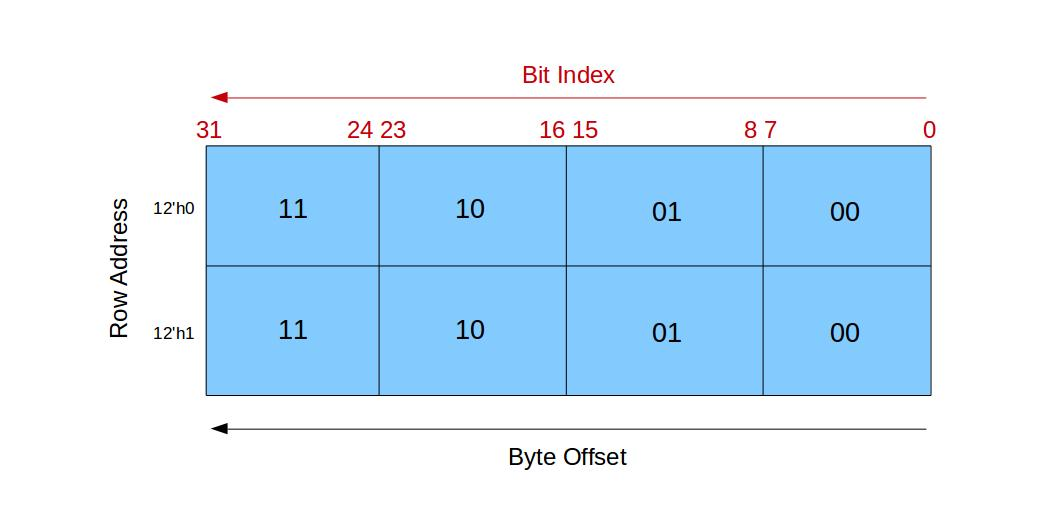
\includegraphics[width=0.6\textwidth]{endianness_img}
    \caption{Block RAM organization. The labels for row address \textbf{should read 14'h0 and 14'h1.}}
    \label{fig:endianness_img}
  \end{center}
\end{figure}

Figure \ref{fig:endianness_img} illustrates the 14-bit word addresses and the two bit byte offsets.
Observe that the RAM organization is \textbf{little-endian}, i.e. the most significant byte is at the most significant memory address (offset '11').

\subsubsection{Reading from RAMs}
Since the RAMs have 32-bit rows, you can only read data out of the RAM 32-bits at a time.
This is an issue when executing an \verb|lh| or \verb|lb| instruction, as there is no way to indicate which 8 or 16 of the 32 bits you want to read out.

Therefore, you will have to shift and mask the output of the RAM to select the appropriate portion of the 32-bits you read out.
For example, if you want to execute a \verb|lbu| on a byte address ending in \verb|2'b10|, you will only want bits \verb|[23:16]| of the 32 bits that you read out of the RAM (thus storing \verb|{24'b0, output[23:16]}| to a register).

\subsubsection{Writing to RAMs}
To take care of \verb|sb| and \verb|sh|, note that the \verb|we| input to the instruction and data memories is 4 bits wide.
These 4 bits are a byte mask telling the RAM which of the 4 bytes to actually write to.
If \verb|we|=\{4'b1111\}, then all 32 bits passed into the RAM would be written to the address given.

Here's an example of storing a single byte:
\begin{itemize}
  \item Write the byte \verb|0xa4| to address \verb|0x10000002| (byte offset = 2)
  \item Set \verb|we = {4'b0100}|
  \item Set \verb|din = {32'hxx_a4_xx_xx}| (\verb|x| means don't care)
\end{itemize}

\subsection{Memory Architecture}
The standard RISC pipeline is usually depicted with separate instruction and data memories.
Although this is an intuitive representation, it does not let us modify the instruction memory to run new programs.
Your CPU, by the end of this checkpoint, will be able to receive compiled RISC-V binaries though the UART, store them into instruction memory, then jump to the downloaded program.
To facilitate this, we will adopt a modified memory architecture shown in Figure \ref{fig:mem_arch}.

\begin{figure}[hbt]
  \begin{center}
    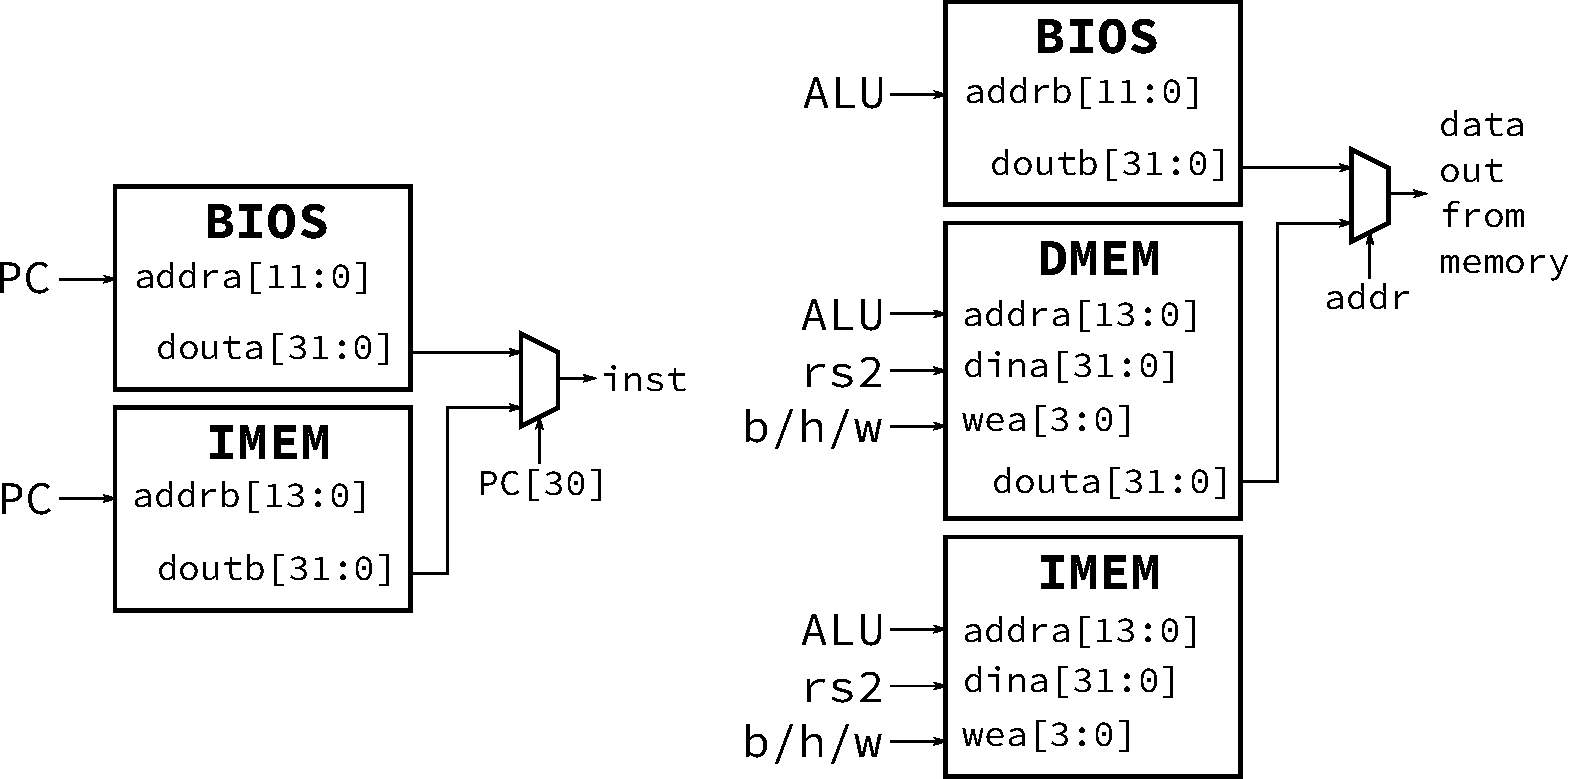
\includegraphics[width=0.8\textwidth]{images/memory_arch.pdf}
    \caption{The Riscv151 memory architecture. There is only 1 IMEM and DMEM instance in Riscv151 but their ports are shown separately in this figure for clarity. The left half of the figure shows the instruction fetch logic and the right half shows the memory load/store logic.}
    \label{fig:mem_arch}
  \end{center}
\end{figure}

\subsubsection{Summary of Memory Access Patterns}
The memory architecture will consist of three RAMs (instruction, data, and BIOS).
The RAMs are memory resources (block RAMs) contained within the FPGA chip, and no external (off-chip, DRAM) memory will be used for this project.

The processor will begin execution from the BIOS memory, which will be initialized with the BIOS program (in \verb|software/bios|).
The BIOS program should be able to read from the BIOS memory (to fetch static data and instructions), and read and write the instruction and data memories.
This allows the BIOS program to receive user programs over the UART from the host PC and load them into instruction memory.

You can then instruct the BIOS program to jump to an instruction memory address, which begins execution of the program that you loaded.
At any time, you can press the reset button on the board to return your processor to the BIOS program.

\subsubsection{Unaligned Memory Accesses}
In the official RISC-V specification, unaligned loads and stores are supported.
However, in your project, you can ignore instructions that request an unaligned access.
Assume that the compiler will never generate unaligned accesses.

\subsubsection{Address Space Partitioning}
Your CPU will need to be able to access multiple sources for data as well as control the destination of store instructions.
In order to do this, we will partition the 32-bit address space into four regions: data memory read and writes, instruction memory writes, BIOS memory reads, and memory-mapped I/O.
This will be encoded in the top nibble (4 bits) of the memory address generated in load and store operations, as shown in Table \ref{mem_space1}.
In other words, the target memory/device of a load or store instruction is dependent on the address.
The reset signal should reset the PC to the value defined by the parameter \verb|RESET_PC| which is by default the base of BIOS memory (\verb|0x40000000|).

\begin{table}[hbt]
  \begin{center}
    \caption{Memory Address Partitions}
    \label{mem_space1}
    \begin{tabular}{l l l l l}
      \bottomrule
      \textbf{Address[31:28]} & \textbf{Address Type} & \textbf{Device} & \textbf{Access} & \textbf{Notes} \\
      \midrule
      4'b00x1 & Data & Data Memory & Read/Write &\\
      4'b0001 & PC  &  Instruction Memory & Read-only &\\
      4'b001x & Data & Instruction Memory & Write-Only & Only if PC[30] == 1'b1\\
      4'b0100 & PC  & BIOS Memory & Read-only &\\
      4'b0100 & Data & BIOS Memory & Read-only &\\
      4'b1000 & Data & I/O & Read/Write &\\
      \bottomrule
    \end{tabular}
  \end{center}
\end{table}

Each partition specified in Table \ref{mem_space1} should be enabled based on its associated bit in the address encoding.
This allows operations to be applied to multiple devices simultaneously, which will be used to maintain memory consistency between the data and instruction memory.

For example, a store to an address beginning with \verb|0x3| will write to both the instruction memory and data memory, while storing to addresses beginning with \verb|0x2| or \verb|0x1| will write to only the instruction or data memory, respectively.
For details about the BIOS and how to run programs on your CPU, see Section~\ref{bios_info}.

Please note that a given address could refer to a different memory depending on which address type it is.
For example the address \verb|0x10000000| refers to the data memory when it is a data address while a program counter value of \verb|0x10000000| refers to the instruction memory.

The note in the table above (referencing PC[30]), specifies that you can only write to instruction memory if you are currently executing in BIOS memory.
This prevents programs from being self-modifying, which would drastically complicate your processor.

\subsubsection{Memory Mapped I/O}
\label{mmio}
At this stage in the project the only way to interact with your CPU is through the UART.
The UART from Lab 5 accomplishes the low-level task of sending and receiving bits from the serial lines, but you will need a way for your CPU to send and receive bytes to and from the UART.
To accomplish this, we will use memory-mapped I/O, a technique in which registers of I/O devices are assigned memory addresses.
This enables load and store instructions to access the I/O devices as if they were memory.

To determine CPI (cycles per instruction) for a given program, the I/O memory map is also used to include instruction and cycle counters.

Table~\ref{mem_map1} shows the memory map for this stage of the project.

\begin{table}[hbt]
  \begin{center}
    \caption{I/O Memory Map}
    \label{mem_map1}
    \begin{adjustbox}{width=\columnwidth,center}
    \begin{tabular}{l l l l}
      \toprule
      \textbf{Address} & \textbf{Function} & \textbf{Access} & \textbf{Data Encoding}\\
      \midrule
      \verb|32'h80000000| & UART control & Read & \verb|{30'b0, uart_rx_data_out_valid, uart_tx_data_in_ready}| \\
      \verb|32'h80000004| & UART receiver data & Read & \verb|{24'b0, uart_rx_data_out}| \\
      \verb|32'h80000008| & UART transmitter data & Write & \verb|{24'b0, uart_tx_data_in}| \\
      \midrule
      \verb|32'h80000010| & Cycle counter & Read & Clock cycles elapsed \\
      \verb|32'h80000014| & Instruction counter & Read & Number of instructions executed \\
      \verb|32'h80000018| & Reset counters to 0 & Write & N/A \\
      \verb|32'h8000001c| & Total branch instruction 
 counter & Read & Number of branch instructions 
 encounted (Checkpoint 3) \\
      \verb|32'h80000020| & Correct branch prediction counter & Read & Number of branches successfully predicted (Checkpoint 3)  \\
      \bottomrule
    \end{tabular}
    \end{adjustbox}
  \end{center}
\end{table}

You will need to determine how to translate the memory map into the proper ready-valid handshake signals for the UART.
Your UART should respond to \verb|sw, sh, and sb| for the transmitter data address, and should also respond to \verb|lw, lh, lb, lhu, and lbu| for the receiver data and control addresses.

You should treat I/O such as the UART just as you would treat the data memory.
This means that you should assert the equivalent write enable (i.e. valid) and data signals at the end of the execute stage, and read in data during the memory stage.
The CPU itself should not check the \verb|uart_rx_data_out_valid| and \verb|uart_tx_data_in_ready| signals; this check is handled in software.
The CPU needs to drive \verb|uart_rx_data_out_ready| and \verb|uart_tx_data_in_valid| correctly.

The cycle counter should be incremented every cycle, and the instruction counter should be incremented for every instruction that is committed (you should not count bubbles injected into the pipeline or instructions run during a branch mispredict).
From these counts, the CPI of the processor can be determined for a given benchmark program.

\subsection{Testing}
\label{testing}
The design specified for this project is a complex system and debugging can be very difficult without tests that increase visibility of certain areas of the design.
In assigning partial credit at the end for incomplete projects, we will look at testing as an indicator of progress.
A reasonable order in which to complete your testing is as follows:

\begin{enumerate}
  \item Test that your modules work in isolation via Verilog testbenches that you write yourself
  \item Test that your CPU pipeline works with the \verb|sim/cpu_tb.v|
  \item Test the entire CPU one instruction at a time with hand-written assembly --- see \verb|sim/asm_tb.v|
  \item Run the \verb|riscv-tests| ISA test suite (\verb|make isa-tests|)
  \item Some extra tests with other software C program, such as \verb|c_tests| and \verb|uart_parse|. They could help reveal more bugs -- see \verb|c_tests_tb.v| and \verb|uart_parse_tb.v|
  \item Test the CPU's memory mapped I/O --- see \verb|echo_tb.v|
  \item Test the CPU's memory mapped I/O with BIOS software program --- see \verb|bios_tb.v|
\end{enumerate}

For more information on testing, please see the README at \verb|hardware/README.md|.

%\subsection{Riscv151 Tests}

%Once you are confident that the individual components of your processor are working in isolation, you will want to test the entire processor as a whole. One way to do this is to pass the \verb|Riscv151_testbench|. To run the test, use either one of the following commands (iverilog is highly recommended since it is faster):\\
%\begin{minted}{bash}

%# Simulate with sim/Riscv151_testbench.v

%# with iverilog
%make iverilog-sim tb=Riscv151_testbench

%# open waveform
%make wave tb=Riscv151_testbench

%# with Vivado
%make sim tb=Riscv151_testbench

%\end{minted}

%The testbench covers all RV32I instructions. To pass this testbench, you should have a working Riscv151 implementation that can decode and execute all the instructions in the spec, including the CSR instructions. Several basic hazard cases are also tested. The testbench does not work with any software code as in the following sections, but rather it manually initializes the instructions and data in the memory blocks as well as the register file content for each test. The testbench does not cover reading from BIOS memory nor memory mapped IO. You will need to complete these components before moving on with other testbenches.

%\subsection{Software Toolchain}
%\label{toolchain}
%A GCC RISC-V toolchain has been built and installed in the eecs151 home directory; these binaries will run on any of the c125m machines in the 125 Cory lab. The \href{https://berkeley.box.com/s/s4z0ykpf0tudrm9hce8fsmitpgb2khhe}{VM Image} also has the toolchain installed along with Vivado 2019.1.

%The most relevant programs in the toolchain are:
%\begin{itemize}
%    \item \verb|riscv64-unknown-elf-gcc|: GCC for RISC-V, compiles C code to RISC-V binaries.
%    \item \verb|riscv64-unknown-elf-as|: RISC-V assembler, compiles assembly code to RISC-V binaries.
%    \item \verb|riscv64-unknown-elf-objdump|: Dumps RISC-V binaries as readable assembly code.
%\end{itemize}

%Look at the \verb|software/c_example| folder for an example of a C program.

%There are several files:
%\begin{itemize}
%    \item \verb|start.s|: This is an assembly file that contains the start of the program.
%      It initialises the stack pointer then jumps to the \verb|main| label.
%      Edit this file to move the top of the stack.
%      Typically your stack pointer is set to the top of the data memory address space, so that the stack has enough room to grow downwards.

%    \item \verb|c_example.ld|: This linker script sets the base address of the program.
%      For Checkpoint 2, this address should be in the format \verb|0x1000xxxx|
%      The .text segment offset is typically set to the base of the instruction memory address space.

%    \item \verb|c_example.elf|: Binary produced after running \verb|make|.\\Use \verb|riscv64-unknown-elf-objdump -Mnumeric -D c_example.elf| to view the assembly code.
%    \item \verb|c_example.dump|: Assembly dump of the binary.
%\end{itemize}

%\subsection{Assembly Tests}
%\label{assembly_tests}
%Hand written assembly tests are in \verb|software/assembly_tests/start.s| and the corresponding testbench is in \verb|hardware/sim/assembly_testbench.v|.
%To run the test, run:\\
%\verb|make sim tb=assembly_testbench|

%\verb|start.s| contains assembly that's compiled and loaded into the BIOS RAM by the testbench.
%\begin{minted}[breaklines]{asm}
%_start:

%# Test ADD
%li x10, 100         # Load argument 1 (rs1)
%li x11, 200         # Load argument 2 (rs2)
%add x1, x10, x11    # Execute the instruction being tested
%li x20, 1           # Set the flag register to stop execution and inspect the result register
%                    # Now we check that x1 contains 300 in the testbench

%Done: j Done
%\end{minted}

%The \verb|assembly_testbench| toggles the clock one cycle at time and waits for register \verb|x20| to be written with a particular value (in the above example: 1).
%Once \verb|x20| contains 1, the testbench inspects the value in \verb|x1| and checks it is 300, which indicates your processor correctly executed the add instruction.

%If the testbench times out it means \verb|x20| never became 1, so the processor got stuck somewhere or \verb|x20| was written with another value.

%You should add your own tests to verify that your processor can execute different instructions correctly. Modify the file \verb|start.s| to add your assembly code, then rerun the RTL simulation.

%\subsection{RISC-V ISA Tests}\label{riscv-isa-tests}
%You will need the CSR instructions to work before you can use this test suite, and you should have confidence in your hand-written assembly tests.
%Test the CSR instructions using hand assembly tests.

%To run the ISA tests, run
%To run the ISA tests, first pull the latest skeleton changes:
%\begin{minted}{bash}
%git pull staff main
%git submodule update --init --recursive
%\end{minted}

%Then run

%\begin{minted}{bash}
%cd hardware

%# with iverilog
%make iverilog-sim tb=isa_testbench test=all

% # with Vivado
% make sim tb=isa_testbench test=all
% \end{minted}

% To run a particular ISA test (e.g. \verb|add|), replace "all" with "add". The simulation should print out which tests passed or failed and their simulation cycles.

% If you're failing a test, debug using the test assembly file in\\\verb|software/riscv-isa-tests/riscv-tests/isa/rv32ui| or the generated assembly dump.
% The assembly dump files are extremely helpful in debugging at this stage. If you look into a particular dump file of a test (e.g., \verb|add.dump|), it contains several subtests in series. The CSR output from the simulation indicates which subtest is failing to help you narrow down where the problem is, and you can start debugging from there.

% The \verb|RESET_PC| parameter is used in \verb|isa_testbench| to start the test in the IMEM instead of the BIOS.
% Make sure you have used it in \verb|Riscv151.v|.

% \subsection{Software Tests}

% \subsubsection{RISC-V Programs}

% Next, you will test your processor with some small RISC-V C programs in \verb|software|.
% We use the RISC-V software toolchain to compile a program to a memory initialization file
% (MIF). The MIF file stores the assembly instructions (encoded in binary format)
% of the program and initializes \texttt{IMem} and \texttt{DMem} in
% \verb|hardware/sim/software_testbench.v| for testing.
% Some available C programs are:

% \verb|software/strcmp/strcmp.c|, \verb|software/vecadd/vecadd.c|,

% \verb|software/fib/fib.c|, \verb|software/sum/sum.c|, \verb|software/replace/replace.c|,

% \verb|software/cachetest/cachetest.c|

% which you can test with the following commands

% \begin{minted}{bash}

% # with iverilog
% make iverilog-sim tb=software_testbench sw=strcmp
% make iverilog-sim tb=software_testbench sw=vecadd
% ...

% # with Vivado
% make sim tb=software_testbench sw=strcmp
% make sim tb=software_testbench sw=vecadd
% ...

% \end{minted}

% These tests could help reveal more hazard bugs in your implementation. \texttt{strcmp} is particular important since it is frequently used in the BIOS program. The tests use CSR instruction to indicate if they are passed (e.g., write '1' to the CSR register if passed). Take a look at the C files for further details. Following that practice, you can also write your custom C program to further test your CPU.

% As an additional tip for debugging, try changing the compiler optimization flag in the \verb|Makefile| of each software test (e.g., \texttt{-O2} to \texttt{-O1} or \texttt{-O0}), or using a newer GCC compiler and see if your processor still passes the test. Different compiler settings generate different sequences of assembly instructions, and some might expose subtle hazard bugs yet to be covered by your implementation.

% \subsubsection{Echo}
% You should have your UART modules integrated with the CPU before running this test. The test verifies if your CPU is able to: check the UART status, read a character from UART Receiver, and write a character to UART Transmitter. Take a look at the software code \verb|software/echo/echo.c| to see what it does. The testbench loads the MIF file compiled from the software code, and load it to the BIOS memory in a similar manner to the assembly test and riscv-isa tests.

% To run the echo test, run

% \begin{minted}{bash}

% # with iverilog
% make iverilog-sim tb=echo_testbench

% # with Vivado
% make sim tb=echo_testbench
% \end{minted}

% The testbench, acts like a host, sends multiple characters via the serial line, then waits until it receives all the characters back. In some sense, it is similar to the echo test in Lab 5, however, the UART modules are controlled by the software program (\verb|software/echo/echo.c|) running on your RISC-V CPU.

% Once you pass the echo test, also try \verb|software/c_test/c_test.c|. This test combines both UART operations and string comparison. It covers the basic functionality of the BIOS program, but is shorter and easier to debug than the BIOS testbench.

% \begin{minted}{bash}

% # with iverilog
% make iverilog-sim tb=c_testbench

% # with Vivado
% make sim tb=c_testbench
% \end{minted}

% \subsection{BIOS and Programming your CPU}
% \label{bios_info}

% We have provided a BIOS program in \verb|software/bios151v3| that allows you to interact with your CPU and download other programs over UART.
% The BIOS is just an infinite loop that reads from the UART, checks if the input string matches a known control sequence, and then performs an associated action.
% For detailed information on the BIOS, see Appendix \ref{sec:biosinfo}.

% Before running the BIOS program on your FPGA, please do the final simulation test with the \verb|sim/bios_testbench.v|. The testbench emulates the interaction between the host and your CPU via the serial lines orchestrated by the BIOS program. It tests four basic functions of the BIOS program: sending invalid command, storing to an address (in \texttt{IMem} or \texttt{DMem}), loading from an address (in \texttt{IMem} or \texttt{DMem}), and jumping to an address (from BIOS to IMem).

% \begin{minted}{bash}

% # with iverilog
% make iverilog-sim tb=bios_testbench

% # with Vivado
% make sim tb=bios_testbench
% \end{minted}

% Once you pass the BIOS testbench, you can implement and test your processor on the FPGA!

% To run the BIOS:
% \begin{enumerate}
%   \item Verify that the stack pointer and .text segment offset are set properly in \verb|start.s| and \verb|bios151v3.ld| in software/bios151v3 directory
%   \item Build a bitstream and program the FPGA. Run \verb|make write-bitstream| in \verb|hardware| to generate a bitstream to your project, then \verb|make program-fpga bs=bitstream_files/z1top.bit| to program the FPGA (if you are programming the FPGA from a lab machine with the Hardware Server, make sure that you update the port number in \verb|hardware/scripts/program_fpga.tcl| to your assigned port number).
%   \item Use screen to access the serial port:
%     \begin{minted}[tabsize=2]{bash}
%     screen $SERIALTTY 115200
%     # or 
%     # screen /dev/ttyUSB0 115200
%     \end{minted}
%   \item Press the reset button to make the CPU PC go to the start of BIOS memory
% \end{enumerate}

% Close screen using \verb|Ctrl-a Shift-k|, or other students won't be able to use the serial port!
% If you can't access the serial port you can run \verb|killscreen| to kill all screen sessions.

% If all goes well, you should see a \verb|151 >| prompt after pressing return. The following commands are available:
% \begin{itemize}
%     \item \verb|jal <address>|: Jump to address (hex).
%     \item \verb|sw, sb, sh <data> <address>|: Store data (hex) to address (hex).
%     \item \verb|lw, lbu, lhu <address>|: Prints the data at the address (hex).
% \end{itemize}

% (if you want to backspace, press \verb|Ctrl + Backspace|)

% As an example, running \verb|sw cafef00d 10000000| should write to the data memory and running \verb|lw 10000000| should print the output \verb|10000000: cafef00d|.
% Please also pay attention that writes to the instruction memory (\verb|sw ffffffff 20000000|) do not write to the data memory, i.e. \verb|lw 10000000| still should yield \verb|cafef00d|.

% In addition to the command interface, the BIOS allows you to load programs to the CPU. \textit{With screen closed}, run:
% \begin{minted}[tabsize=2]{bash}
%     scripts/hex_to_serial <mif_file> <address>
% \end{minted}

% This stores the \verb|.mif| file at the specified hex address.
% In order to write into both the data and instruction memories, \textbf{remember to set the top nibble to 0x3}

% (i.e. \verb|scripts/hex_to_serial echo.mif 30000000|, assuming the \verb|.ld| file sets the base address to \verb|0x10000000|).

% You also need to ensure that the stack and base address are set properly (See Section \ref{toolchain}).
% For example, before making the \verb|mmult| program you should set the set the base address to \verb|0x10000000| (see \ref{mmult}).
% Therefore, when loading the \verb|mmult| program you should load it at the base address: \verb|scripts/hex_to_serial mmult.mif 30000000|.
% Then, you can jump to the loaded \verb|mmult| program in in your screen session by using \verb|jal 10000000|.

% \subsection{Target Clock Frequency}
% By default, the CPU clock frequency is set at 50MHz.
% It should be easy to meet timing at 50 MHz.
% Look at the timing report to see if timing is met.
% If you failed, the timing reports specify the critical path you should optimize.

% For this checkpoint, we will allow you to demonstrate the CPU working at 50 MHz, but for the final checkoff at the end of the semester, you will need to optimize for a higher clock speed ($\geq$ 100MHz) for full credit.
% Details on how to build your FPGA design with a different clock frequency will come later.

% \subsection{Matrix Multiply}
% \label{mmult}
% To check the correctness and performance of your processor we have provided a benchmark in \verb|software/mmult/| which performs matrix multiplication.
% You should be able to load it into your processor in the same way as loading the echo program.

% This program computes $S=AB$, where $A$ and $B$ are 64$\times$64 matrices.
% The program will print a checksum and the counters discussed in Section ~\ref{mmio}.
% The correct checksum is \verb|0001f800|.
% If you do not get this, there is likely a problem in your CPU with one of the instructions that is used by the BIOS but not mmult.

% The matrix multiply program requires that the stack pointer and the offset of the .text segment be set properly, otherwise the program will not execute properly.

% The stack pointer (set in \verb|start.s|) should start near the top of DMEM to avoid corrupting the program instructions and data.
% It should be set to \verb|0x1000fff0| and the stack grows downwards.

% The .text segment offset (set in \verb|mmult.ld|) needs to accommodate the full set of instructions and static data (three 64$\times$64 matrices) in the mmult binary.
% It should be set to the base of DMEM: \verb|0x10000000|.

% The program will also output the values of your instruction and cycle counters (in hex).
% These can be used to calculate the CPI for this program.
% Your target CPI should not be greater than 1.2.
% If your CPI exceeds this value, you will need to modify your datapath and pipeline to reduce the number of bubbles inserted for resolving control hazards (since they are the only source of extra latency in our processor).
% This might involve performing naive branch prediction or moving the jalr address calculation to an earlier stage.

\subsection{How to Succeed in This Checkpoint}
Start early and work on your design incrementally.
Draw up a very detailed and organised block diagram and keep it up to date as you begin writing Verilog.
Unit test independent modules such as the control unit, ALU, and regfile.
Write thorough and complex assembly tests by hand, and don't solely rely on the RISC-V ISA test suite.
The final BIOS program is several 1000 lines of assembly and will be nearly impossible to debug by just looking at the waveform.

The most valuable asset for this checkpoint will not be your GSIs but will be your fellow peers who you can compare notes with and discuss design aspects with in detail.
However, do NOT under any circumstances share source code.

Once you're tired, go home and \textit{sleep}. When you come back you will know how to solve your problem.

\subsubsection{How to Get Started}
It might seem overwhelming to implement all the functionality that your processor must support. The best way to implement your processor is in small increments, checking the correctness of your processor at each step along the way. Here is a guide that should help you plan out Checkpoint 1 and 2:

\begin{enumerate}
  \item \textit{Design.} You should start with a comprehensive and detailed design/schematic. Enumerate all the control signals that you will need. Be careful when designing the memory fetch stage since all the memories we use (BIOS, instruction, data, IO) are synchronous.
  \item \textit{First steps.} Implementing some modules that are easy to write and test.
  \item \textit{Control Unit + other small modules.} Implement the control unit, ALU, and any other small independent modules. Unit test them.
  \item \textit{Memory.} In the beginning, only use the BIOS memory in the instruction fetch stage and only use the data memory in the memory stage. This is enough to run assembly tests.
  \item \textit{Connect stages and pipeline.} Connect your modules together and pipeline them. At this point, you should be able to run integration tests using assembly tests for most R and I type instructions.
  \item \textit{Implement handling of control hazards.} Insert bubbles into your pipeline to resolve control hazards associated with JAL, JALR, and branch instructions. Don't worry about data hazard handling for now. Test that control instructions work properly with assembly tests.
  \item \textit{Implement data forwarding for data hazards.} Add forwarding muxes and forward the outputs of the ALU and memory stage. Remember that you might have to forward to ALU input A, ALU input B, and data to write to memory. Test forwarding aggressively; most of your bugs will come from incomplete or faulty forwarding logic. Test forwarding from memory and from the ALU, and with control instructions.
  \item \textit{Add BIOS memory reads.} Add the BIOS memory block RAM to the memory stage to be able to load data from the BIOS memory. Write assembly tests that contain some static data stored in the BIOS memory and verify that you can read that data.
  \item \textit{Add Inst memory writes and reads.} Add the instruction memory block RAM to the memory stage to be able to write data to it when executing inside the BIOS memory. Also add the instruction memory block RAM to the instruction fetch stage to be able to read instructions from the inst memory. Write tests that first write instructions to the instruction memory, and then jump (using jalr) to instruction memory to see that the right instructions are executed.
  \item \textit{Run Riscv151\_testbench}. The testbench verifies if your Riscv151 is able to read the RV32I instructions from instruction memory block RAM, execute, and write data to either the Register File or data memory block RAM.
  \item \textit{Run isa\_testbench}. The testbench works with the RISCV ISA tests. This comprehensive test suites verifies the functionality of your processor.
  \item \textit{Run software\_testbench}. The testbench works with the software programs under \verb|software| using the CSR check mechanism as similar to the \verb|isa_testbench|. Try testing with all the supported software programs since they could expose more hazard bugs.
  \item \textit{Add instruction and cycle counters.} Begin to add the memory mapped IO components, by first adding the cycle and instruction counters. These are just 2 32-bit registers that your CPU should update on every cycle and every instruction respectively. Write tests to verify that your counters can be reset with a \verb|sw| instruction, and can be read from using a \verb|lw| instruction.
  \item \textit{Integrate UART.} Add the UART to the memory stage, in parallel with the data, instruction, and BIOS memories. Detect when an instruction is accessing the UART and route the data to the UART accordingly. Make sure that you are setting the UART ready/valid control signals properly as you are feeding or retrieving data from it. We have provided you with the \verb|echo_testbench| which performs a test of the UART. In addition, also test with \verb|c_testbench| and \verb|bios_testbench|.
  \item \textit{Run the BIOS.} If everything so far has gone well, program the FPGA. Verify that the BIOS performs as expected. As a precursor to this step, you might try to build a bitstream with the BIOS memory initialized with the echo program.
  \item \textit{Run matrix multiply.} Load the \verb|mmult| program with the \verb|hex_to_serial| utility (located under \texttt{scripts/}), and run \verb|mmult| on the FPGA. Verify that it returns the correct checksum.
  \item \textit{Check CPI.} Compute the CPI when running the \verb|mmult| program. If you achieve a CPI 1.2 or smaller, that is acceptable, but if your CPI is larger than that, you should think of ways to reduce it.
\end{enumerate}

\subsection{Checkoff}
The checkoff is divided into two stages: block diagram/design and implementation.
The second part will require significantly more time and effort than the first one.
As such, completing the block diagram in time for the design review is crucial to your success in this project.

\subsubsection{\blockDiagramTaskName}
\textbf{Block Diagram}\\
The first checkpoint requires a detailed block diagram of your datapath.
The diagram should have a greater level of detail than a high level RISC datapath diagram.
You may complete this electronically or by hand.

If working by hand, we recommend working in pencil and combining several sheets of paper for a larger workspace.
If doing it electronically, you can use Inkscape, Google Drawings, draw.io or any program you want.

You should be able to describe in detail any smaller sub-blocks in your diagram.
\textbf{Though the diagrams from textbooks/lecture notes are a decent starting place, remember that they often use asynchronous-read RAMs for the instruction and data memories, and we will be using synchronous-read block RAMs}.

Additionally, you will be asked to provide short answers to the following questions based on how you structure your block diagram. The questions are intended to make you consider all possible cases that might happen when your processor execute instructions, such as data or control hazards. It might be a good idea to take a moment to think of the questions first, then draw your diagram to address them.

\textbf{Questions}\label{sec:chkpt1_questions}
\begin{enumerate}
\item How many stages is the datapath you've drawn? (i.e. How many cycles does it take to execute 1 instruction?)
\item How do you handle ALU $\rightarrow$ ALU hazards?

addi x1, x2, 100

addi x2, x1, 100

\item How do you handle ALU $\rightarrow$ MEM hazards?

addi x1, x2, 100

sw x1, 0(x3)

\item How do you handle MEM $\rightarrow$ ALU hazards?

lw x1, 0(x3)

addi x1, x1, 100

\item How do you handle MEM $\rightarrow$ MEM hazards?

lw x1, 0(x2)

sw x1, 4(x2)

also consider:

lw x1, 0(x2)

sw x3, 0(x1)

\item Do you need special handling for 2 cycle apart hazards?

addi x1, x2, 100

 nop

 addi x1, x1, 100

\item How do you handle branch control hazards? (What is the mispredict latency, what prediction scheme are you using, are you just injecting NOPs until the branch is resolved, what about data hazards in the branch?)
\item How do you handle jump control hazards? Consider jal and jalr separately. What optimizations can be made to special-case handle jal? 
\item What is the most likely critical path in your design?
\item Where do the UART modules, instruction, and cycle counters go? How are you going to drive \verb|uart_tx_data_in_valid| and \verb|uart_rx_data_out_ready| (give logic expressions)?
\item What is the role of the CSR register? Where does it go?
\item When do we read from BIOS for instructions? When do we read from IMem for instructions? How do we switch from BIOS address space to IMem address space? In which case can we write to IMem, and why do we need to write to IMem? How do we know if a memory instruction is intended for DMem or any IO device?
\end{enumerate}

Commit your block diagram and your writeup to your team repository under \verb|fa22_fpga_teamXX/docs| by \blockDiagramDueDate. Please also remember to push your working IO circuits to your GitHub repository.

\subsubsection{\baseCPUTaskName: Base RISCV151 System}
This checkpoint requires a fully functioning three stage RISC-V CPU as described in this specification.
Checkoff will consist of a demonstration of the BIOS functionality, loading a program (\verb|echo| and \verb|mmult|) over the UART, and successfully jumping to and executing the program.

Additionally, please find the maximum achievable frequency of your CPU implementation. To do so, lower the \verb|CPU_CLOCK_PERIOD| (starting at 20, with a step size of 1) in \verb|hardware/src/z1top.v| until the Implementation fails to meet timing. Please report the critical path in your implementation.

\textbf{\baseCPUTaskName \space materials should be committed to your project repository by \baseCPUDueDate.}

\subsubsection{Checkpoints 1 \& 2 Deliverables Summary}
\begin{center}
  \begin{tabular}{m{45mm} m{40mm} m{70mm}}
    \toprule
    \textbf{Deliverable} & \textbf{Due Date \newline(for all sections)} & \textbf{Description} \\
    \midrule
    Block Diagram, RISC-V ISA Questions, IO code & \blockDiagramDueDate & Push your block diagram, your write-up, and IO code to your GitHub repository. \linebreak In-lab Checkoff: Sit down with a GSI and go over your design in detail. \\
    \midrule
    RISC-V CPU, Fmax and Crit. path & \baseCPUDueDate & Check in code to GitHub. \linebreak In-lab Checkoff: Demonstrate that the BIOS works, you can use \verb|hex_to_serial| to load the \verb|echo| program, \verb|jal| to it from the BIOS, and have that program successfully execute. Load the mmult program with \verb|hex_to_serial|, \verb|jal| to it, and have it execute successfully and return the benchmarking results and correct checksum. Your CPI should not be greater than 1.2\\
    \bottomrule
  \end{tabular}
\end{center}

\pagebreak

% \section{Checkpoint 3 - Hardware-Accelerated Convolutional Neural Network}

% \subsection{Checkpoint Overview}

% \subsubsection{LeNet}

% In this checkpoint, your task is to design and implement an optimized hardware accelerator to speed up the inference execution of a small Convolutional Neural Network (CNN). You will be comparing the performance of your accelerator against the CNN software implementation running on the RISC-V processor that you have implemented in Checkpoint 2. Our target CNN is the classic \href{http://yann.lecun.com/exdb/lenet/}{LeNet-5} network for handwritten digit classification. LeNet-5 is a feed-forward network that consists of 5 layers as shown in the following figure.

% \begin{center}
% 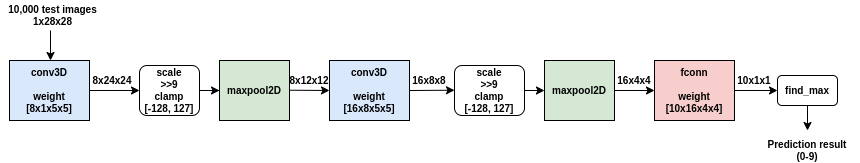
\includegraphics[width=0.8\textwidth]{images/lenet.png}
% \end{center}

% A rigorous understanding of deep neural networks is not required when you do this checkpoint, since we will provide the software model of the problem. Nonetheless, if you'd like to look at some introductory materials to get yourself acquainted with some Deep learning concepts, the \href{https://inst.eecs.berkeley.edu/~eecs151/sp21/files/EECS251Leture-JennyHuang_2021.pdf}{Deep Neural Networks Design and Examples} lecture or the lecture notes from \href{https://inst.eecs.berkeley.edu//~ee290-2/sp21/}{EE290-2} are good places to start.

% Here are some key parameters of the network. We refer an input matrix to a layer as input feature map (IFM), and the output matrix of a layer as output feature map (OFM).

% \begin{itemize}
% \item The first 3D Convolutional layer (conv3D): input feature map 1$\times$28$\times$28 (8-bit), weight 8$\times$1$\times$5$\times$5 (8-bit), output feature map 8$\times$24$\times$24 (32-bit)
% \item The first 2D Max Pooling layer (maxpool2D): input feature map 8$\times$2$\times$24 (32-bit), output feature map 8$\times$12$\times$12 (8-bit)
% \item The second 3D Convolutional layer: input feature map 8$\times$12$\times$12 (8-bit), weight 16$\times$8$\times$5$\times$5 (8-bit), output feature map 16$\times$8$\times$8 (32-bit)
% \item The second 2D Max Pooling layer: input feature map 16$\times$8$\times$8 (32-bit), output feature map 16$\times$4$\times$4 (8-bit)
% \item The Fully-Connected layer (fconn): input feature map 16$\times$4$\times$4 (8-bit), weight 10$\times$16$\times$4$\times$4 (8-bit), output feature map 10$\times$1$\times$1 (32-bit)
% \end{itemize}

% The network is trained with the MNIST dataset to obtain the weight data for the two conv3D layers and fconn layers. The weights, initially in floating-point datatype, are then quantized to 8-bit signed integers (-128 to 127) to reduce the implementation complexity (no floating-point computation required) as well as make the network leaner and more FPGA-friendly. The general consensus is that the inference does not need a lot of bits to achieve competitive accuracy to full precision as opposed to the training process. The output feature maps of these layers are also quantized to 8-bit signed integers by being scaled down by a factor of 512 and clamped to within the range of -128 to 127. The quantization has negligible impact on the accuracy of the network (97\% on 10000 MNIST test images). This technique is called Post-training quantization. The Python script for training the network is adapted from the \href{https://drive.google.com/file/d/1LBtLjz2pdo6uj-E0aR69-ZGjmR9RBSDU/view}{Lab 1 material} of the course EE290-2.

% You might have noticed that the network is small enough that we could fit all the weight data of these layers on our PYNQ-Z1. This is not always possible for state-of-the-art neural networks. To make the problem more challenging and practical, the quantized weights, along with the 10000 quantized test images are initialized on the off-chip DRAM of the PYNQ-Z1 platform. Therefore, data won't simply be initialized in any on-chip Memory blocks and embedded in the bitstream as we've done so far, instead extra efforts must be done to bring the data closer to your computational units.

% This checkpoint gives you a different design problem from what was asked in checkpoint 2, since now you will need to build a specialized datapath for computation and memory buffering optimized specifically for this application. You are free to use any modules you like (memory blocks, FIFOs) for your design as long as everything is working correctly and faster than the baseline (naive) implementation. There is also no restriction on the amount of memory storage for your accelerator design.

% From the previous lab and homework execises, you have already had some practice on mapping an algorithmic description of a problem (e.g., loop forms) into a circuit implementation. To that end, this checkpoint furthers the complexity in terms of the number of loop levels and the amount of operations needed to carry out per loop iteration. How do a software loop iteration and a hardware cycle correlate? Would it be possible to map one or more software loop iterations to one hardware cycle? Can we overlap the operations of current loop iteration with the next one? Can we unroll the loops to achieve higher degree of parallelism? Can we partition a memory module such that we are not constrained by the number of available memory ports for parallel read/write? Bring all the design techniques that you have learned from the lectures with you, and see how far you can get with your accelerator design.

% \subsubsection{New files}
% Please do \textbf{git pull staff main} to get the latest updates for this checkpoint from the staff repository. Some new files have been added:

% \begin{itemize}
% \item \verb|hardware/src/z1top_axi.v|: New top-level module to integrate with the Zynq Processing System IP. We will use this top module from now on for the project.
% \item \verb|hardware/src/accelerator/xcel_naive.v|: An accelerator with a naive conv3D implementation. You will use this as the baseline.
% \item \verb|hardware/src/accelerator/xcel_naive_compute.v|: The compute unit of \verb|xcel_naive|. It implements a conv3D operation.
% \item \verb|hardware/src/accelerator/xcel_naive_memif.v|: The memory interface unit of \verb|xcel_naive|. It handles bus read/write to the DRAM and services the request/response from the compute unit.
% \item \verb|hardware/src/accelerator/xcel_opt.v|: A skeleton code for the optimized accelerator module. \textbf{Your task is to complete this file}.
% \item \verb|hardware/src/accelerator/axi_mm_adapter.v|: An AXI Memory-Mapped (MM) master adapter core for interfacing with the Zynq Processing System.
% \item \verb|hardware/src/accelerator/axi_mm_read.v|: A sub-component of the AXI MM adapter that implements the AXI read logic.
% \item \verb|hardware/src/accelerator/axi_mm_write.v|: A sub-component of the AXI MM adapter that implements the AXI write logic.
% \item \verb|hardware/src/accelerator/dma_controller.v|: A DMA (Direct-Memory Access) controller for interfacing with the off-chip DRAM and the RISC-V Data Memory (\texttt{DMem}) via the AXI adapter.
% \item \verb|hardware/src/accelerator/arbiter.v|: An arbiter for selecting which client (DMA or Accelerator) to service requests and responses to and from the off-chip DRAM.
% \item \verb|hardware/sim/xcel_testbench.v|: A testbench for verifying the functionality of the \verb|xcel| implementation. Only conv3D operation is tested.
% \item \verb|hardware/sim/conv3D_testbench.v|: A testbench for verifying the functionality of the compute unit \verb|xcel_naive_compute|. Only conv3D operation is tested.
% \item \verb|hardware/sim/mem_model.v|: A simple memory model that works with the \verb|xcel_testbench.v|.
% \item \verb|software/axi_test/*|: Software files for testing AXI communication (read and write).
% \item \verb|software/lenet/*|: Software files for the LeNet inference demo.
% \end{itemize}

% \subsubsection{High-level Overview of the Full System}
% The following figure depicts the overall picture of the full system.

% \begin{center}
% 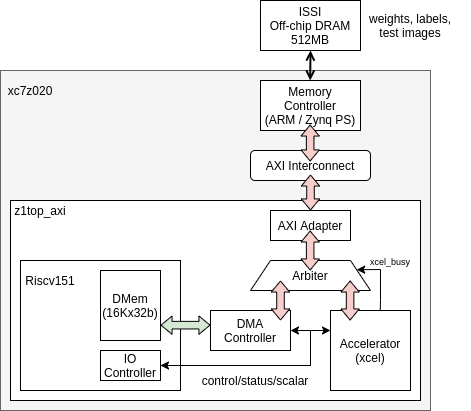
\includegraphics[width=0.5\textwidth]{images/full_system.png}
% \end{center}

% The DMA Controller orchestrates the memory communication between the RISC-V's \texttt{DMem} and the off-chip DRAM. The AXI adapter receives a write or read request from either the DMA or the Accelerator, and submits the request to the off-chip DRAM through the Zynq Processing System. The arbiter implements a simple MUXing logic to service the request and response from the Accelerator if it is currently running, otherwise the DMA. Note that there is no direct memory transfer between the RISC-V and the Accelerator. All memory communication must go through the off-chip DRAM. For example, if the Accelerator wants to read some data from the RISC-V's \texttt{DMem} block, it must be first transferred to a memory location of the off-chip DRAM by the DMA, and the data can be accessed at the specified DRAM address by the read logic implemented inside the Accelerator. Similarly, any result data computed by the Accelerator must also be written to the DRAM before the RISC-V core can read it. The operations of the DMA and the Accelerator are controlled by the IO controller inside the Riscv151 core. To the Riscv151 core's perspective, they act as IO devices as similar to the UART modules.

% \subsubsection{ARM Baremetal Application}

% A pre-compiled ARM binary is provided to initialize the off-chip DRAM with the weight, image, and label data.

% \begin{center}
% 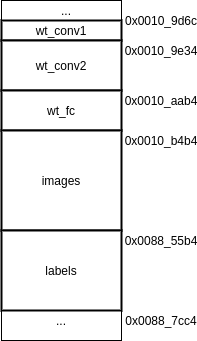
\includegraphics[width=0.2\textwidth]{images/ddr_layout.png}
% \end{center}

% You can take a look at the C source file \verb|arm_baremetal_app/system/helloworld.c| to see how things are set up. In order to compile this application, you will need to have access to a different Xilinx software (Vivado SDK). However, since the application is pre-compiled, you do not need to worry about this. You don't even need to touch any of the files in this submodule when doing the checkpoint. The addresses of the weight, image, and label data are statically allocated as shown in the DRAM memory layout figure above (only showing the data section). We will provide these addresses to the DMA Controller and the Accelerator so that they can access to the correct locations of the DRAM to get the data. Since ARM uses byte-level addressing scheme, a 32-bit read from the memory retrieves four consecutive 8-bit data items (e.g., weights).

% \subsection{Software Implementation}

% This section provides the software description for the computational kernels found in our network: conv3D, maxpool2D, and fconn. You are not required to implement all these computational kernels in your accelerator, although you're welcome to do so. The bare minimum requirement is that you must accelerate the 3D Convolutional function as similar to the naive accelerator implementation given to you.

% To keep things simple, your conv3D module is only required to handle convolution with a stride of 1 and no padding. Therefore, no boundary check is necessary. In addition, the weight dimension is passed as a parameter to the Verilog module (statically known). You're encourage to write your code in a parameterizable manner since it is a good coding practice (i.e., no assumption on the value of the weight dimension), but this is not strictly compulsory.

% \subsubsection{conv3D}

% \begin{center}
% 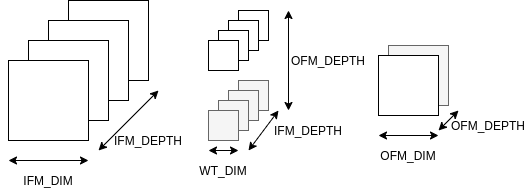
\includegraphics[width=0.5\textwidth]{images/conv3D.png}
% \end{center}

% \begin{minted}[fontsize=\footnotesize]{C}
% // Since the stride is 1 and no padding required, OFM_DIM = IFM_DIM - WT_DIM + 1

% #define OFM_SIZE  (OFM_DIM * OFM_DIM)
% #define IFM_SIZE  (IFM_DIM * IFM_DIM)
% #define WT_SIZE   (WT_DIM * WT_DIM)
% #define WT_VOLUME (IFM_DEPTH * WT_SIZE)

% for (f = 0; f < OFM_DEPTH; f++) {

%   for (i = 0; i < OFM_DIM; i++) {
%     for (j = 0; j < OFM_DIM; j++) {
%       ofm[f * OFM_SIZE + i * OFM_DIM + j] = 0;
%     }
%   }

%   for (d = 0; d < IFM_DEPTH; d++) {
%     for (i = 0; i < OFM_DIM; i++) {
%       for (j = 0; j < OFM_DIM; j++) {
%         int32_t tmp = 0;
%         for (m = 0; m < WT_DIM; m++) {
%           for (n = 0; n < WT_DIM; n++) {
%             int32_t ifm_data = ifm[d * IFM_SIZE + (i + m) * IFM_DIM + (j + n)];
%             int32_t wt_data  = wt[f * WT_VOLUME + d * WT_SIZE + m * WT_DIM + n];
%             tmp += ifm_data * wt_data;
%           }
%         }

%         ofm[f * OFM_SIZE + i * OFM_DIM + j] += tmp;
%       }
%     }
%   }
% }

% \end{minted}

% \newpage
% \subsubsection{maxpool2D}

% \begin{minted}[fontsize=\footnotesize]{C}
% #define OFM_DIM  (IFM_SIZE / 2)
% #define OFM_SIZE (OFM_DIM * OFM_DIM)
% #define IFM_SIZE (IFM_DIM * IFM_DIM)

% for (f = 0; f < OFM_DEPTH; f++) {
%   for (i = 0; i < OFM_DIM; i++) {
%     for (j = 0; j < OFM_DIM; j++) {
%       int8_t tmp0 = ifm[d * IFM_SIZE + (i*2+0) * IFM_DIM + (j*2+0)];
%       int8_t tmp1 = ifm[d * IFM_SIZE + (i*2+1) * IFM_DIM + (j*2+0)];
%       int8_t tmp2 = ifm[d * IFM_SIZE + (i*2+0) * IFM_DIM + (j*2+1)];
%       int8_t tmp3 = ifm[d * IFM_SIZE + (i*2+1) * IFM_DIM + (j*2+1)];

%       tmp0 = (tmp0 > 0) ? tmp0 : 0;
%       tmp1 = (tmp1 > 0) ? tmp1 : 0;
%       tmp2 = (tmp2 > 0) ? tmp2 : 0;
%       tmp3 = (tmp3 > 0) ? tmp3 : 0;

%       ofm[f * OFM_SIZE + i * OFM_DIM + j] = max(tmp0, tmp1, tmp2, tmp3);
%     }
%   }
% }

% \end{minted}

% %\newpage
% \subsubsection{fconn}

% \begin{minted}[fontsize=\footnotesize]{C}
% // In some sense, a fully-connected operation can also be view as conv3D
% // with WT_DIM == IFM_DIM (and OFM_DIM = 1)

% #define WT_DIM    (IFM_DIM)
% #define IFM_SIZE  (IFM_DIM * IFM_DIM)
% #define WT_SIZE   (WT_DIM * WT_DIM)
% #define WT_VOLUME (IFM_DEPTH * WT_SIZE)

% for (f = 0; f < OFM_DEPTH; f++) {
%   int32_t tmp = 0;
%   for (d = 0; d < IFM_DEPTH; d++) {
%     for (i = 0; i < IFM_DIM; i++) {
%       for (j = 0; j < IFM_DIM; j++) {
%         int32_t ifm_data = ifm[d * IFM_SIZE + i * IFM_DIM + j];
%         int32_t wt_data  = wt[f * WT_VOLUME + d * WT_SIZE + i * WT_DIM + j];
%         tmp += ifm_data * wt_data;
%       }
%     }
%   }
%   ofm[f] += tmp;
% }

% \end{minted}

% \newpage
% \subsection{Naive conv3D: Sources of Inefficiency}

% A straight mapping from a software description to a hardware implementation, without considering many inherent characteristics of the system (memory latency, buffering, available compute blocks, etc.), undoubtedly yields poor result. Have a look at the baseline conv3D implementation given to you: \verb|hardware/src/accelerator/xcel_naive.v|. There are a few weaknesses in this implementation.

% \begin{itemize}
% \item This implementation reads the elements of input feature map redundantly without considering the fact that there are some overlap between the current and the next sliding window (with a stride of 1). Therefore, the off-chip memory latency quickly overwhelms the performance and leaves the compute unit starving for data most of the time.
% \item This implementation does not consider the fact that the weight and input feature map are 8-bit data, and that 4 weight/IFM items could be packed in a single read transfer at a time since our AXI data bus is 4 times wider. Instead, it issues 4 separate single read transfers for those consecutive weight/IFM data items. The redundancy adds extra communication overhead.
% \item This implementation does not utilize burst mode to achieve better memory bandwidth utilization, especially since there are multiple data items in a row and one could set up a burst request to read them all in successive cycles with some intial startup overhead from the request to the response.
% \item This implementation does not utilize any intermediate buffer to store the partial compute results on chip. Instead, the partial output channel result (OFM) is written back to the DRAM, and then read again to accumulate with the next result.
% \item Per sliding window computation, the weight and the IFM data are preloaded into shift registers, then a single multiply-accumulation (MAC) operation is performed per cycle of the sliding window. However, one could also fully unroll this computation to use more MAC operations to compute a sliding window in a cycle with the trade-off of more hardware resource.
% \item The FSM design serializes the execution and leaves small room to achieve pipelining or overlapping between memory fetching/writing and computation. The FSM embeds the mental model of the sequential software execution. Can we redesign or get rid of the FSM to achieve better pipelining execution of memory fetch/write and computation?
% \end{itemize}

% To build an efficient accelerator, one needs to not only understand how the software code works, but also be able to transform it to some form that is hardware-friendly in terms of memory access patterns, data reuses, and parallel executions. The topic of CNN acceleration has been extensively studied and explored, so we won't have any issues of finding some existing architecture to implement for the checkpoint. Nonetheless, you're also welcome to pursue your own ideas.

% \subsection{AXI Bus Interface}

% This section intends to provide you some background on the ARM's AMBA AXI bus interface.
% AXI is a widely popular standard interface for establishing and standardizing the communication between many IP cores.
% Our communication cores (DMA, Accelerator, AXI Adapter) adopt the AXI4 interface bus protocol.
% There are separate read/write request and response channels.
% Per each channel, a handshake mechanism (Ready/Valid) is used to indicate a successful transaction.

% You can skim the official ARM's AXI specification \href{https://developer.arm.com/documentation/ihi0022/b}{here} for more information (chapter 2, 3, and 4).
% The reading is entirely optional. The following subsections give a brief summary on the protocol and things that are particularly important for this checkpoint.
% Additional resource is Xilinx \href{https://www.xilinx.com/support/documentation/ip\_documentation/ug761\_axi\_reference\_guide.pdf}{AXI Reference Guide}.

% To reduce the design complexity, our AXI data bus width is set to 32-bit to match with the data word width of the RISC-V processor. And similar to our processor core, the Zynq PS uses byte-level addressing. A read from a DRAM memory location retrieves 4 consecutive bytes on the data bus. Likewise, a write to a memory location will update all 4 bytes. There's also a write strobe signal to set which byte lane(s) of the data bus to write to the memory.

% The AXI read/write logic to interface with the Zynq PS is provided to you:

% \verb|hardware/src/accelerator/axi_mm_adapter.v|.

% One of your responsibilities in \verb|hardware/src/accelerator/xcel_opt.v| is to figure out how to set up the read and write interface channels to the AXI Adapter core so that your accelerator can read or write data correctly from and to the off-chip DRAM.

% \subsubsection{Read Interface Channels}

% \textbf{1. Read Address Request channel}
% \begin{itemize}
% \item \textbf{araddr}: Memory read request address (output)
% \item \textbf{arvalid}: Memory read request address valid signal (output)
% \item \textbf{arready}: Memory read request address ready signal (input)
% \item \textbf{arlen}: Memory read burst length (output): the number of data transfers per read transaction (offset by 1).
% \item \textbf{arsize}: Memory read burst size (output): the number of bytes per data transfer (log based 2).
% \item \textbf{arburst}: Memory read burst type (output). Set to \textit{INCREMENT} so that the bus receives successive data items in a row.
% \end{itemize}

% \textbf{2. Read Data Response channel}
% \begin{itemize}
% \item \textbf{rdata}: Memory read response data (input)
% \item \textbf{rvalid}: Memory read response data valid signal (input)
% \item \textbf{rready}: Memory read response data ready signal (output)
% \item \textbf{rlast}: Memory read response data last signal (input). Stays HIGH on the last data transfer.
% \end{itemize}

% Figure ~\ref{fig:axi_read} demonstrates an example of an AXI read transaction.
% A read request is submitted, and a burst of 4 data beats are sent to the read response data channel.

% Figure ~\ref{fig:axi_read_burst} shows the timings of the relevant AXI signals on a read transaction. Note how handshake is used to indicate when we have a fired request or response data (valid and ready are both HIGH at a rising clock edge).

% \begin{figure}[hbt]
% \begin{center}
%   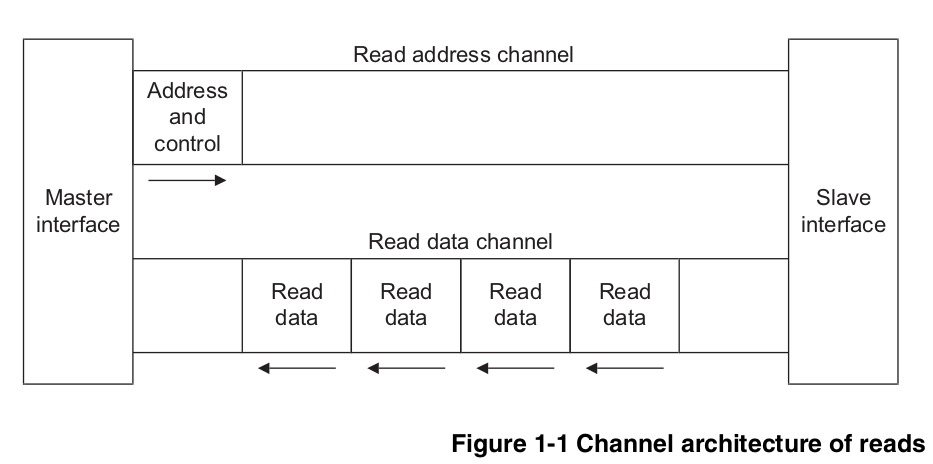
\includegraphics[width=0.6\textwidth]{axi_read.png}
%   \caption{An AXI read transaction. Source: \href{https://developer.arm.com/documentation/ihi0022/b}{AXI Spec}}
%   \label{fig:axi_read}
% \end{center}
% \end{figure}

% \begin{figure}[hbt]
% \begin{center}
%   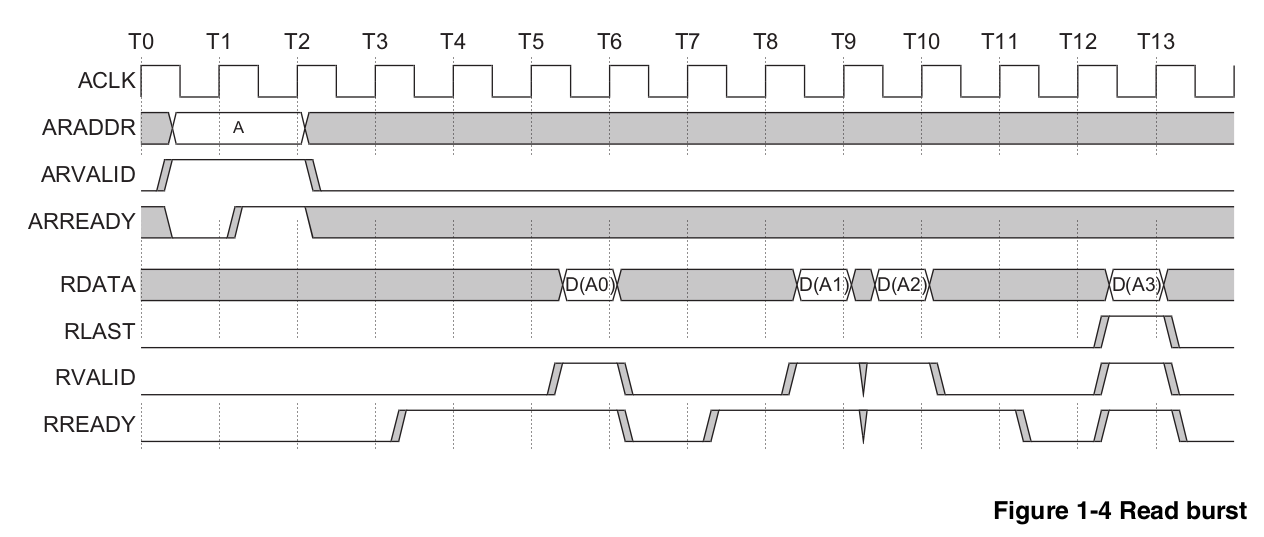
\includegraphics[width=0.6\textwidth]{axi_read_burst.png}
%   \caption{An AXI read burst timing diagram. Source: \href{https://developer.arm.com/documentation/ihi0022/b}{AXI Spec}}
%   \label{fig:axi_read_burst}
% \end{center}
% \end{figure}

% \subsubsection{Write Interface Channels}

% \textbf{1. Write Address Request channel}
% \begin{itemize}
% \item \textbf{awaddr}: Memory write request address (output)
% \item \textbf{awvalid}: Memory write request address valid signal (output)
% \item \textbf{awready}: Memory write request address ready signal (output)
% \item \textbf{awlen}: Memory write burst length (output): the number of data transfers per read transaction (offset by 1).
% \item \textbf{awsize}: Memory write burst size (output): the number of bytes per data transfer (log based 2).
% \item \textbf{awburst}: Memory write burst type (output). Set to \textit{INCREMENT} so that the bus receives successive data items in a row.
% \end{itemize}

% \textbf{2. Write Data Request channel}
% \begin{itemize}
% \item \textbf{wdata}: Memory write request data (output)
% \item \textbf{wvalid}: Memory write request data valid (output)
% \item \textbf{wready}: Memory write request data ready (input)
% \item \textbf{wlast}: Memory write request data last (output). Set to HIGH on the last write data transfer.
% \item \textbf{wstrb}: Memory write request data strobe (output). Set to 4'b1111 if writing the full word to the DRAM memory.
% \end{itemize}

% \textbf{3. Write Response channel}
% \begin{itemize}
% \item \textbf{bresp}: Memory write response (input). The value \textit{RESP\_OKAY} (4'b0000) indicates a write sucess.
% \item \textbf{bvalid}: Memory write response valid signal (input)
% \item \textbf{bready}: Memory write response ready signal (output)
% \end{itemize}

% Figure ~\ref{fig:axi_write} demonstrates an example of an AXI write transaction.
% A write request is submitted, and a burst of 4 data beats are sent to the write data channel.

% Figure ~\ref{fig:axi_write_burst} shows the timings of the relevant AXI signals on a write transaction. Also note how handshake is used to indicate when we have a fired request or response.

% \begin{figure}[hbt]
% \begin{center}
%   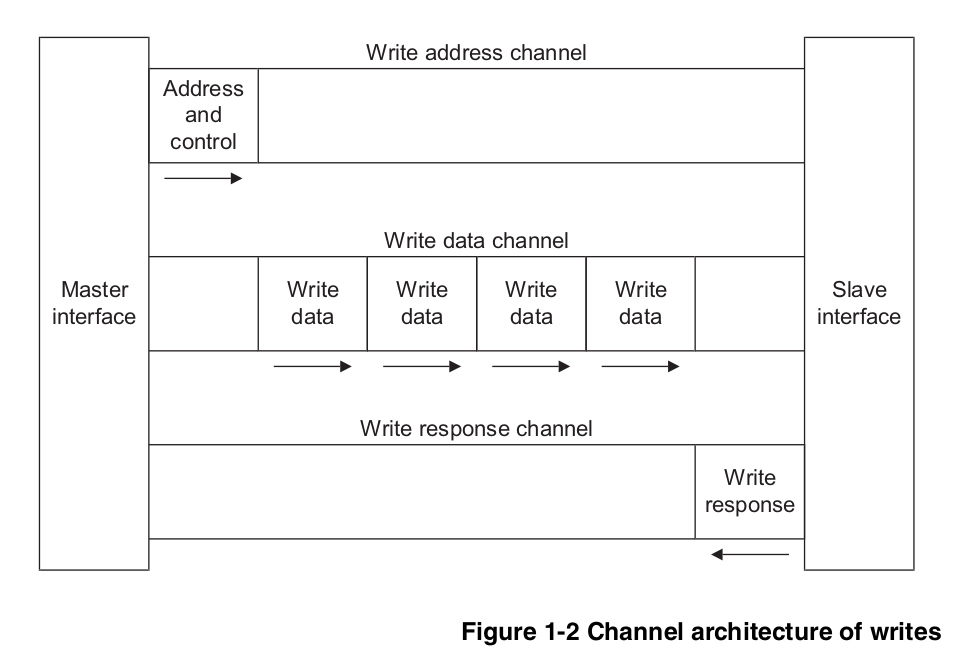
\includegraphics[width=0.6\textwidth]{axi_write.png}
%   \caption{An AXI write transaction. Source: \href{https://developer.arm.com/documentation/ihi0022/b}{AXI Spec}}
%   \label{fig:axi_write}
% \end{center}
% \end{figure}

% \begin{figure}[hbt]
% \begin{center}
%   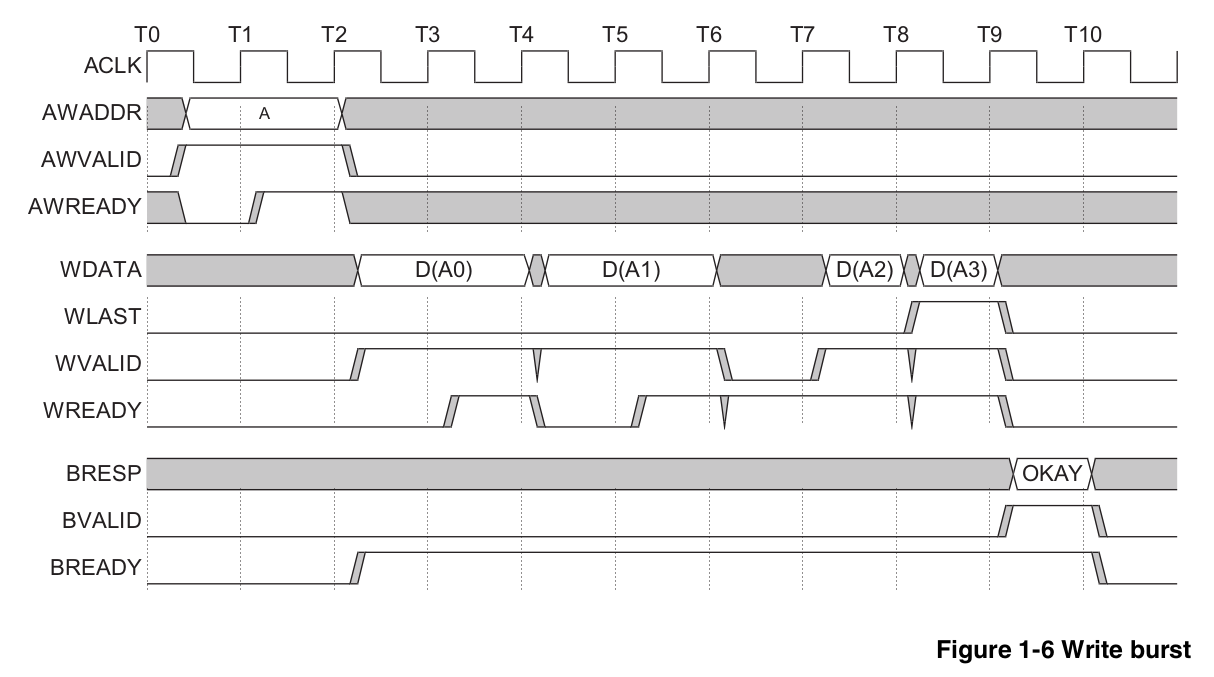
\includegraphics[width=0.6\textwidth]{axi_write_burst.png}
%   \caption{An AXI write burst timing diagram. Source: \href{https://developer.arm.com/documentation/ihi0022/b}{AXI Spec}}
%   \label{fig:axi_write_burst}
% \end{center}
% \end{figure}

% \newpage
% \subsection{Vivado Block Design with Zynq Processing System (PS)}

% \begin{figure}[hbt]
% \begin{center}
%   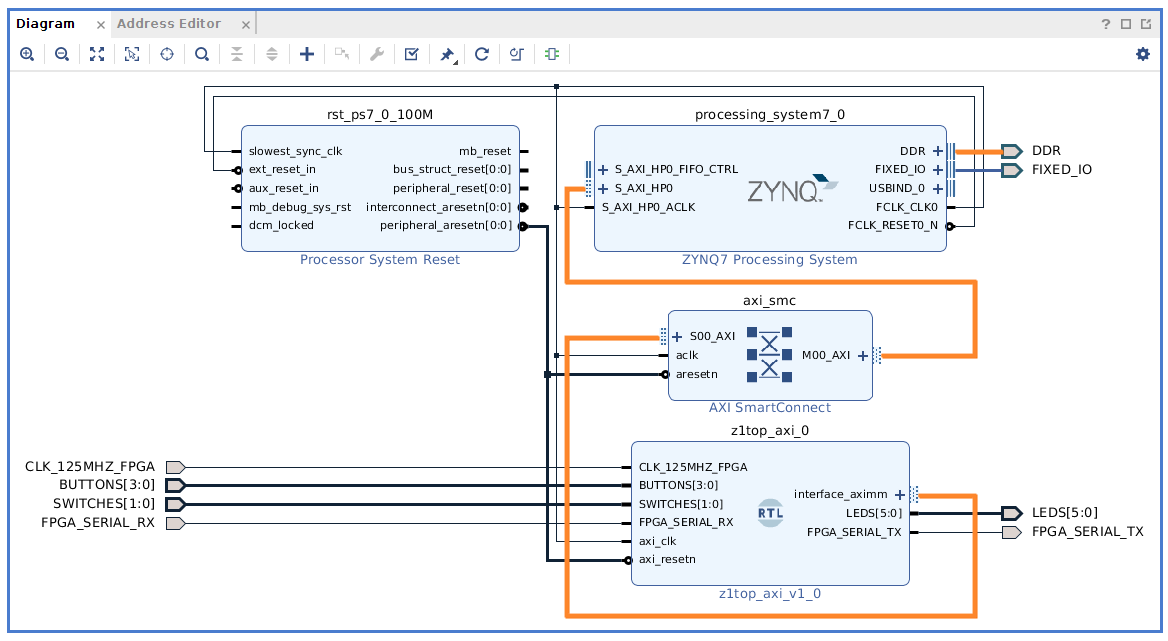
\includegraphics[width=0.7\textwidth]{images/vivado_bd_z1top_axi.png}
%   \caption{The Block Design of z1top\_axi module with the Zynq PS}
%   \label{fig:z1top_axi}
% \end{center}
% \end{figure}

% Figure ~\ref{fig:z1top_axi} shows the Block design of the full system after running the following command.

% \begin{minted}{bash}
% make build-project proj=z1top_axi
% \end{minted}

% Our \verb|z1top_axi.v| communicates with the Zynq PS through the AXI SmartConnect IP using the AXI4 bus interface. The Zynq PS also serves as a memory controller to the off-chip DRAM. Therefore, the only way for a module implemented in the Programmable Logic (PL) to access to the DRAM is through the Zynq PS. A High Performance AXI port (HP0) is used to communicate with the PL. The Zynq PS can be configured to use up to 4 HPs (HP0-3) to increase the memory bandwidth. For the sake of simplicity, we only use one HP port.

% Also note that the Zynq PS supplies the clock signal \verb|FCLK_CLK0| to the fabric modules. To avoid extra timing complexity concerning with multi-clock domains, we will not use our usual \verb|CLK_FPGA_125MHZ|, but rather rely on the clock signal from the PS to clock the synchronous logic of our implementation.

% If you are curious as how to build the project manually with the GUI, refer to the Appendix \ref{sec:vivado_bd} for the details.

% \subsection{System Integration with Riscv151}
% \subsubsection{Memory-mapped IO (MMIO) Registers of the DMA Controller and the Accelerator}

% You will need to extend your IO memory-mapped logic to integrate the DMA controller and the Accelerator (xcel) cores to Riscv151. We will use the load and store instructions to the memory-mapped IO registers as a mechanism to control (start) or check the status of these IO modules (idle, done) as similar to how we have done it with the UART modules in Checkpoint 2. The done signal should be kept HIGH once the \texttt{dma} or \texttt{xcel} finishes, since a software code will keep polling on this signal (busy-waiting) before moving to the next part of the program. In addition, we introduce additional memory-mapped registers to set various address offsets so that the cores know where to access the correct data in any memory devices (DRAM or \texttt{DMem}). This is a neat approach to avoid hard-coding the addresses or recompiling the whole bitstream everytime we change the memory layout of the software/application code. The input/output feature map dimension and depth can also be set in software code.

% The addresses of the MMIO registers are defined in \verb|software/151_library/memory_map.h|.

% \begin{table}[hbt]
%   \begin{center}
%     \caption{MMIO addresses for the DMA Controller and the Accelerator}
%     \label{mem_map_dma_xcel}
%     \begin{adjustbox}{width=\columnwidth,center}
%     \begin{tabular}{l l l l}
%       \toprule
%       \textbf{Address} & \textbf{Function} & \textbf{Access} & \textbf{Data Encoding}\\
%       \midrule
%       \verb|32'h80000030| & dma control (start) & Write & N/A \\
%       \verb|32'h80000034| & dma status & Read & \verb|{30'b0, idle, done}| \\
%       \verb|32'h80000038| & dma direction (1: \texttt{DMem} to DRAM, 0: DRAM to \texttt{DMem}) & Write & \verb|{31'b0, direction}| \\
%       \verb|32'h8000003c| & dma source address & Write & DMA source address (32-bit) \\
%       \verb|32'h80000040| & dma destination address & Write & DMA destination address (32-bit) \\
%       \verb|32'h80000044| & dma transfer length (per 4 bytes) & Write & DMA transfer length (32-bit) \\
%       \verb|32'h80000050| & xcel control (start) & Write & N/A \\
%       \verb|32'h80000054| & xcel status & Read & \verb|{30'b0, idle, done}| \\
%       \verb|32'h80000058| & xcel input feature map DRAM address & Write & IFM DRAM address (32-bit) \\
%       \verb|32'h8000005c| & xcel weight DRAM address & Write & WT DRAM address (32-bit) \\
%       \verb|32'h80000060| & xcel output feature map DRAM address & Write & OFM DRAM address (32-bit) \\
%       \verb|32'h80000064| & xcel input feature map dimension & Write & IFM dimension value (32-bit) \\
%       \verb|32'h80000068| & xcel input feature map depth (number of channels) & Write & IFM depth value (32-bit) \\
%       \verb|32'h8000006c| & xcel output feature map dimension & Write & OFM dimension value (32-bit) \\
%       \verb|32'h80000070| & xcel output feature map depth (number of channels) & Write & OFM depth value (32-bit) \\
%       \bottomrule
%     \end{tabular}
%     \end{adjustbox}
%   \end{center}
% \end{table}


% \subsubsection{Integrating DMA Controller with CPU Data Memory}

% You might have already noticed that this system would not work with the current setting of Riscv151 in that \texttt{DMem} is a single-port memory block. In addition, port a is currently being used for the CPU load and store instructions. We would need to do the following steps to integrate the DMA Controller safely to the existing system.

% \begin{itemize}
% \item Use a dual-port memory template for \texttt{DMem} (look at \texttt{IMem} as an example)
% \item Connect port b of \texttt{DMem} to the Memory interface of the DMA Controller (via Riscv151).
% \end{itemize}

% This will enable the DMA Controller to have access to the Data Memory.

% \subsection{LeNet Demo software code}

% The FPGA demo of this checkpoint is to run the software code \verb|software/lenet| on your RISC-V processor. The demo runs the LeNet inference to perform handwritten digit classification of the first 128 test images from the MNIST dataset. The demo can be compiled to run with either software flow (running the entire LeNet on the RISC-V) or the hardware-software partition/hybrid flow (executing the two conv3D layers on the accelerator, and the rest of the LeNet on RISC-V). In the software flow, the DRAM-read DMA operations are carried out to first fetch all the weight data to \texttt{DMem} of the RISC-V core. A test image is also fetched from the DRAM to \texttt{DMem} before running the network. The output feature map results of each layer are written to the arrays allocated in \texttt{DMem} and read by the next layer. Our \texttt{DMem} is large enough to hold the weights and the OFM results of the layers in addition to a single test image.

% The hardware/software partition flow, on the other hand, performs the conv3D operation in the hardware accelerator (\texttt{xcel}). By supplying the weight and image addresses in the DRAM, the accelerator knows where to get the data and performs its computation. The output feature map result is written back to the DRAM at an address specified in software (e.g., \verb|0x00900000|). The data is then read by the DMA to \texttt{DMem} since the Max Pooling layers are executed on RISC-V.

% \begin{center}
% 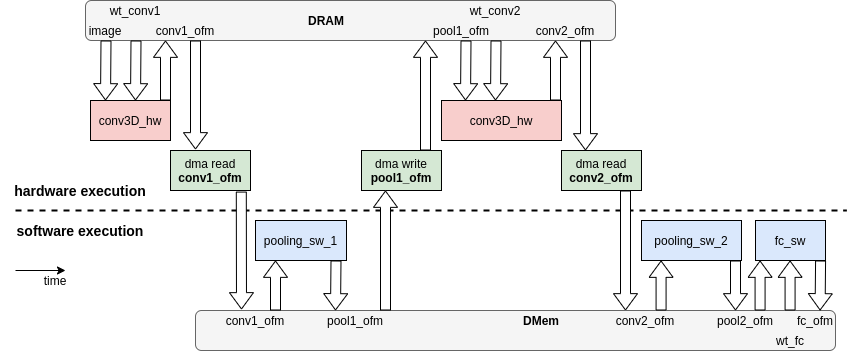
\includegraphics[width=0.7\textwidth]{images/lenet_hybrid_flow.png}
% \end{center}

% In practice, you could implement an accelerator that computes all the layers with intermediate buffers to store the OFMs, so that no DMA operation is needed to copy data back-and-forth between the DRAM and \texttt{DMem}, therefore reducing the number of off-chip memory accesses. Please feel free to change the hardware/software partition flow in accordance with your accelerator design and implementation.

% \newpage
% \subsection{Steps to Complete Checkpoint 3}

% First, get the latest changes from the project skeleton repo

% \begin{minted}{bash}
% git pull staff main
% git submodule update --init --recursive
% \end{minted}

% This will clone the \verb|arm_baremetal_app| submodule.

% The next step is integrating the \texttt{dma\_controller} and \texttt{xcel\_naive} to your existing Riscv151 processor.
% First, you need to modify the interface of \verb|hardware/src/riscv_core/Riscv151.v| to include some additional input/output ports to connect to the DMA controller and the Accelerator as follows.

% \newpage
% \begin{minted}[fontsize=\footnotesize]{Verilog}
% module Riscv151 #(
%   parameter CPU_CLOCK_FREQ = 50_000_000,
%   parameter RESET_PC       = 32'h4000_0000,
%   parameter BAUD_RATE      = 115200,
%   parameter BIOS_MIF_HEX   = "bios151v3.mif"
% ) (
%   input  clk,
%   input  rst,
%   input  FPGA_SERIAL_RX,
%   output FPGA_SERIAL_TX,
%   output [31:0] csr,

%   // Accelerator Interfacing
%   output xcel_start,
%   input xcel_done,
%   input xcel_idle,

%   output [31:0] ifm_ddr_addr,
%   output [31:0] wt_ddr_addr,
%   output [31:0] ofm_ddr_addr,

%   output [31:0] ifm_dim,
%   output [31:0] ifm_depth,

%   output [31:0] ofm_dim,
%   output [31:0] ofm_depth,

%   // DMA Interfacing
%   output dma_start,
%   input  dma_done,
%   input  dma_idle,
%   output dma_dir,
%   output [31:0] dma_src_addr,
%   output [31:0] dma_dst_addr,
%   output [31:0] dma_len,

%   // DMem Interfacing (Port b)
%   input  [13:0] dmem_addrb,
%   input  [31:0] dmem_dinb,
%   output [31:0] dmem_doutb,
%   input  [3:0]  dmem_web,
%   input         dmem_enb
% );
% \end{minted}

% You need to expand your IO memory-mapped logic to perform load/store to the memory addresses of these IO modules as mentioned in the section above,
% so that the CPU can control them from software. In addition, you will also need to convert \texttt{DMem} to dual-port memory block.
% Use \texttt{port b} to connect to the \texttt{dma\_controller} via the interface of the Riscv151 processor.
% Don't forget to wire the enable port of \texttt{DMem} to \texttt{dmem\_enb} from the interface.
% Also note that we're no longer using \verb|hardware/src/z1top.v| for this checkpoint, but \verb|hardware/src/z1top_axi.v| instead.

% Once you finish the integration, don't forget to rerun the simulation of all the tests from Checkpoint 2 to make sure that the new changes don't accidentally introduce bugs to your processor.

% Next, generate a bitstream to configure your FPGA. Now you can pass the target clock frequency to the command.

% \begin{minted}{bash}
% # This command will implement and generate bitstream
% # for the z1top_axi module and set the clock period to 20ns
% make write-bitstream proj=z1top_axi clk=20
% \end{minted}

% Next, before programming the FPGA, you need to run the following script to initialize the Zynq PS (init the clock signal and the DRAM).

% \begin{minted}{bash}
% # If you are programming the FPGA from a lab machine with the Hardware Server,
% # make sure that you update the port number in
% # hardware/scripts/init_arm.tcl to your assigned port number.
% # This script only needs to run once when you first turn on the board,
% # or when your bitstream is implemented with a new clock period
% make init-arm

% # Program the board
% make program-fpga bs=bitstream_files/z1top_axi.bit
% \end{minted}

% Next, test the DRAM communication with your Riscv151 to verify that you have integrated the DMA correctly. There is a software program for that \verb|software/axi_test|. Run the program using the same command as in \texttt{mmult} case. Alternatively, you can do

% \begin{minted}{bash}
% cd software/axi_test
% make run
% \end{minted}

% Next, open the screen program as usual, then do \verb|jal 10000000|.

% This program sends an array allocated in \texttt{DMem} of your RISC-V core to a memory location in the DRAM (DMA write operation), and reads from that memory location (DMA read operation) and writes the result to a different array in \texttt{DMem}. There should not be any mismatches between the two arrays once the DMA finishes. Try testing with different transfer lengths or addresses.

% If the DMA is working, you can move on to the next part, which is to run the LeNet software. Go to \verb|software/lenet|, and run the program as follows.

% \begin{minted}{bash}
% # This will compile and run the hardware implementation of LeNet (only conv3D is
% # put in hardware)
% make clean && make xcel=HW
% make run
% # This will compile and run the software implementation of LeNet
% make clean && make
% make run

% # You can also use the hex_to_serial script to load the generate MIF file
% # to the UART as in the mmult demo

% \end{minted}

% Open screen and then do \verb|jal 10000000| to execute the program.
% The program tests 128 images with 127 correct predictions (\verb|0x0000007f|).
% The failed prediction is at the image \verb|0x00000073| with a prediction of 9
% while the groundtruth is 4. The groundtruth labels can be checked \href{https://github.com/EECS150/arm_baremetal_app/blob/main/system/src/labels.h}{here}.

% You can also test with fewer images (change the macro \verb|NUM_TEST_IMAGES| in \verb|lenet.c|) to make the program run a little faster.

% Once you get a sense of how the entire flow works, it's time to code your own accelerator!
% You can use the naive code as a starting point, but please feel free to write your own code for everything.
% Add your own implementation to \verb|xcel_opt.v|, then replace the naive module with the opt module
% in \verb|z1top_axi.v|.

% \subsection{Resources and Suggestions for Accelerator design}

% You are encouraged to visit the \href{http://eyeriss.mit.edu/tutorial.html}{MIT DNN Eyeriss tutorial} for ideas on how to build the accelerator for the 3D Convolution operation or CNN in general. The DNN Accelerators slides: \href{http://www.rle.mit.edu/eems/wp-content/uploads/2019/06/Tutorial-on-DNN-05-DNN-Accelerator-Architectures.pdf}{Part 1} and \href{http://www.rle.mit.edu/eems/wp-content/uploads/2019/06/Tutorial-on-DNN-06-RS-Dataflow-and-NoC.pdf}{Part 2} are particularly informative and might be useful for you as a starting point (check the \textit{Row-stationary architecture}).

% You can also design a conv2D accelerator and augment it to compute 3D Convolution. As an example, the conv2D engine shown in the following figure fully unrolls the sliding-window computation kernel. Each Processing Element (PE) holds one row of a weight channel in a shift register, and performs a conv1D operation with a row fetched from the IFM, then buffers the result to a FIFO in order to accumulate with the result computed by the next PE. The general idea is that a conv2D operation can be accomplished by doing a conv1D operation separately on each row of a weight channel, then accumulate the result. The final accumulated value is written to the OFM buffer. This convolution architecture achieves two primary optimizations: i) \textbf{parallelization} due to unrolling -- the PEs compute their own conv1D concurrently without any synchronization overhead due to the use of intermediate FIFO buffers; ii) \textbf{data reuse} -- the weight data is reused throughout one conv2D execution, and an IFM data item is only fetched and used once across all the PE, therefore, no redundant data is read from the memory. This architecture is also suitable for streaming execution which the input to the engine can be a FIFO buffer or any streaming interface.

% \begin{center}
% 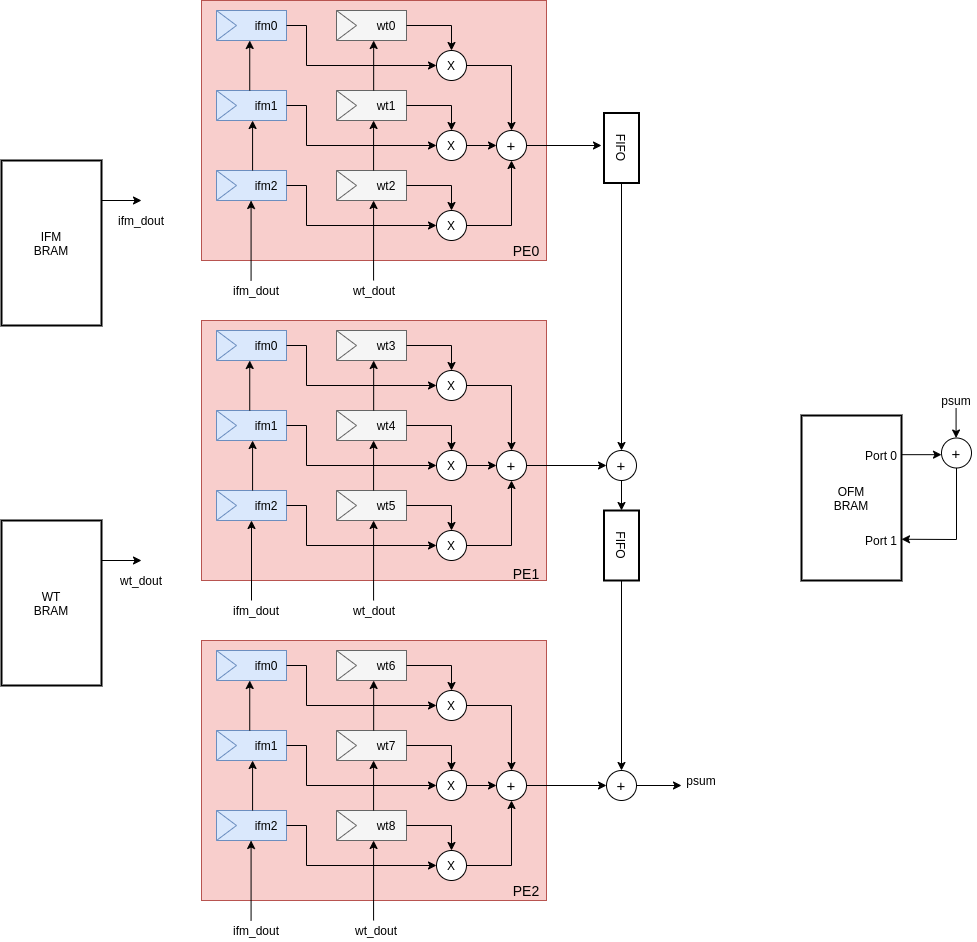
\includegraphics[width=0.7\textwidth]{images/conv2D_engine.png}
% \end{center}

% On the performance estimation, barring a few cycles due to the overhead of filling the shift registers (both IFM and WT) at the beginning or when transitioning from one row to the next, the engine should be able to complete one OFM (partial) channel (or conv2D) in roughly \verb|OFM_SIZE| cycles. One could as well instantiates multiple conv2D engines to compute more OFM (partial) channels in parallel.

% The slides \href{https://drive.google.com/file/d/1SJ6eUK9qJZXzZpeHY_D31d1M95nZMTjR/view?usp=sharing}{\textbf{here}} shows some detailed cycle-by-cycle operations of the engine and might be able to give you some ideas to get started.

% Alternatively, start with something simple that works first, then worry about optimization later. It makes sense to just copy all the weight data and a test image to on-chip BRAM before you start doing the computatation. Buffering the temporary result to another local buffer, and only writing back to the DRAM once everything is done. Using burst mode is highly recommended. As a reference, you can take a look at the code in \verb|hardware/src/accelerator/dma_controller.v| to see some examples of how to setup a burst read/write request, and then how to convert the AXI interface to the RAM interface (i.e., \verb|addr|, \verb|din|, \verb|dout|, \verb|we|) and vice versa. You could do something similar to that in your accelerator. When implementing the bus read/write logic, adopt good practice when it comes to handshake: don't wire ready to valid or vice versa. Another good practice is to modularize the design to two modules as similar to the naive implementation: compute unit and memory interface unit. The memory interface unit handles reading and writing data to the DRAM, while the compute unit performs some computation (e.g., conv3D). For the compute unit, simplify the interface (e.g., RAM interface) so that it allows you to concentrate on implementing and testing the functionality of the computation core.

% Once you have the data on chip, the low-hanging fruit is doing some unrolling or pipelining for parallel execution. Make use of dual-port memory modules to allow you to have more parallel accesses. In addition, try not to use a monolithic memory for everything, but instead split it to smaller modules and assign one for each compute unit.

% As an additional tip for debugging, you can take advantage of Vivado Integrated Logic Analyzer, especially when you debug your AXI read and write logic in your accelerator design. Check the Appendix \ref{sec:vivado_ila} for more detail. Nonetheless, don't rely too much on ILA since it would add extra time to the already arduous Place-and-Route process. The best way to debug is still writing your own testbenches and doing RTL simulation before you run Vivado implementation. A testbench for conv3D has been provided to you. Please feel free to use or change the testbench as you see fit.

% \begin{minted}{bash}
% cd hardware
% make iverilog-sim tb=xcel_testbench
% \end{minted}

% The testbench does not invoke any software MIF file nor the RISC-V core that you designed in Checkpoint 2. Rather, it tests the functionality of the xcel accelerator (conv3D) with a simple \verb|hardware/sim/mem_model.v| in place. A memory block is instantiated in the memory model to initialize data for testing. There's also another testbench that verifies the functionality of the compute unit only (excluding the memory interface logic). You may want to use these testbenches when you design and implement your optimized \verb|xcel| module. Start by implementing a compute module that passes \verb|conv3D_testbench| first, then add a memory interface module to handle bus read/write logic, and finally put everything together to test with \verb|xcel_testbench|. Please feel free to modify these testbenches to fit your own needs.

% \begin{minted}{bash}
% cd hardware
% make iverilog-sim tb=conv3D_testbench
% \end{minted}

% If you would like to start from the naive version, you could try optimizing one unit at a time so that it becomes less overwhelming when you implement and debug your design. For example, start with the naive memory unit module: add burst mode or local memory buffers for memory optimization. Keep the naive compute unit module intact, then simulate with the \verb|xcel_testbench|, and test on the board to verify that your memory optimization works correctly. Once you're confident about your optimized memory unit, the next step is optimizing the compute unit. The decoupled or handshake interface between the given compute and the memory modules, as illustrated in the following figure, allows us to modularize the accelerator design to focus on doing and testing one thing at a time, which to a greater extent help ease the debugging effort. Note that, here \verb|addr| and \verb|ready| are used to signify a memory read equest from the compute unit to the memory interface unit, while \verb|dout| along with \verb|valid| are the memory read response from the memory interface unit to the compute module. On the other hand, \verb|din|, \verb|addr|, and \verb|valid| combines to a memory write request to the memory interface module.

% \begin{center}
% 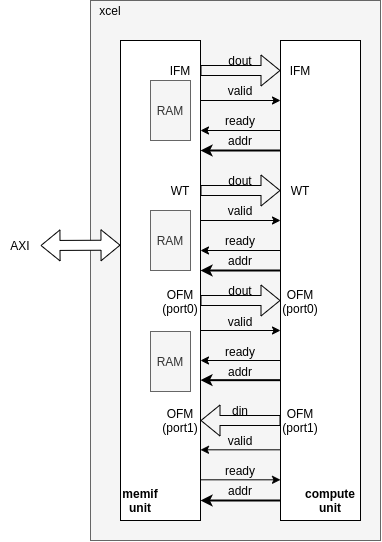
\includegraphics[width=0.3\textwidth]{images/compute_memif.png}
% \end{center}

% Once you have everything working, you can further simplify your implementation by removing the handshake mechanism if your compute unit only retrieves or writes data to some local buffers whose the access latency is statically known.

% Regarding the choices of buffers for memory optimization, you may use your own FIFO modules, or \verb|ASYNC_RAM| / \verb|SYNC_RAM| module templates from \verb|hardware/src/EECS151.v| depending on your implementation. However, recall in Lab 3 and lectures, an \verb|ASYNC_RAM| gets mapped to the LUTRAM, while a \verb|SYNC_RAM| is synthesized to BRAM on the FPGA. Typically, LUTRAMs makes sense for implementing small data storage such as a $32\times32$ Register File in your RISC-V processor. At a greater scale and density, a BRAM would be a more appropriate choice and would help your design achieve much better QoR in terms of area and maximum achievable frequency. Note that on our PYNQ-Z1 platform, there are 17400$\times$64b LUTRAM cells in total, while the number of 36Kb BRAM cells is 140. You should do the calculation and budget your memory allocation appropriately to make sure that your design can accommodate the amount of data that you decide to fetch from the DRAM to on-chip storage.

% When doing on-board testing (running the LeNet code on your FPGA), you may want to use the checksum functions (\verb|checksum_i32()| and \verb|checksum_i8()| in \verb|software/lenet/lenet.c|) to verify if your implementation works correctly (similar to \texttt{mmult} case). Set \textit{NUM\_TEST\_IMAGES} to 1 to test with only the first image. The prediction result is 7, and below are the checksums of the OFM returned by each layer

% \begin{itemize}
% \item conv1\_ofm: \verb|0x005a3760| (calculated with \verb|checksum_i32()|)
% \item pool1\_ofm: \verb|0x00002d6b| (calculated with \verb|checksum_i8()|)
% \item conv2\_ofm: \verb|0xff41b202| (calculated with \verb|checksum_i32()|)
% \item pool2\_ofm: \verb|0x00001451| (calculated with \verb|checksum_i8()|)
% \item fc\_ofm: \verb|0xffffa09a| (calculated with \verb|checksum_i32()|)
% \end{itemize}

% Here is an example of how to calculate the checksum of the OFM result computed by the first conv3D layer.

% \newpage
% \begin{minted}{C}
% // Perform conv3D on the accelerator
% // Write the OFM result to DDR at address 0x90_0000
% conv3D_hw(IMAGES_DDR_ADDR + i * IMG_SIZE, WT_CONV1_DDR_ADDR, 0x900000,
%           IMG_DIM, IMG_DEPTH, CV1_DIM, CV1_DEPTH);
% // Read the OFM result (computed by the accelerator) to the
% // local conv1_ofm in RISC-V DMem
% dma_read_ddr(0x900000, (uint32_t)conv1_ofm >> 2, CONV1_OFM_SIZE);
% int32_t chksum = checksum_i32(conv1_ofm, CONV1_OFM_SIZE);
% uwrite_int8s("\r\nChecksum: ");
% uwrite_int8s(uint32_to_ascii_hex(chksum, buffer, BUF_LEN));
% uwrite_int8s("\r\n");
% \end{minted}

% If you are unsure why your prediction result is different from the expectation, try to isolate the problem by verifying the checksum of your accelerator execution against the software version at each layer of the network.

% As ever, always refer to the Synthesis log file as an additional means for debugging, especially if your implementation passes the simulation (and you're sure that you have rigorously simulated it with different testcases), but fails to run correctly on the FPGA. The simulator takes the behavioral description (in Verilog) of your circuit as input, and that behavioral description gets translated to circuit netlist after Synthesis; functional mismatches could occur due to many reasons, so you should inspect the log file and check all the suspicious warnings. As we are using Block Design flow in this checkpoint, the Synthesis log file that you should pay attention to is located here \verb|z1top_axi_proj/z1top_axi_proj.runs/z1top_axi_bd_z1top_axi_0_0_synth_1/runme.log|.

% Please also feel free to add extra parameters to your accelerator. You need to change the MMIO addresses in software and your Riscv151 IO controller to support the new parameters.

% Should you need to make changes to any of the files given to you, either to make your implementation more efficient or functioning, please feel free to do so.

% \newpage
% \subsection{Checkpoint 3 Deliverables Summary}

% In-lab Checkoff: Demonstrate that your accelerator implementation \verb|xcel_opt| works correctly with the \textit{lenet} software, i.e. it should produce a result that matches the software implementation when testing with the first 128 images from the MNIST dataset. You should be able to obtain some speedup over the given baseline \verb|xcel_naive| implementation. There is no target speedup for the checkpoint as long as you implement some memory optimization (e.g., buffering) and compute optimization (e.g., loop unrolling, pipelining) for your accelerator.

% Additionally, please write a short report (push to \textit{docs/}) with your answers to the following questions
% \begin{itemize}
% \item Sketch the block diagram of your accelerator design. What memory and compute optimizations would you like to highlight in your design?
% \item What is the speedup of your optimized accelerator on testing 128 images over the software execution in terms of \textbf{cycle count}? What about the baseline (naive) accelerator implementation?
% \item Where do you think the speedup comes from? What makes the software (CPU) execution so inefficient in comparison to the specialized hardware implementation?
% \item The RV32I instruction set encoding implemented in our Riscv151 does not have a multiply instruction. Therefore, a multiplication is carried out by a software routine instead (look at the \textbf{times} function in \verb|mmult/mmult.c| as well as \verb|lenet/cnn.c|). Can you come up with an approach to implement a \textit{multiply operation} for your processor (that should be more efficient than invoking \textbf{times} function)? You don't have to implement it, just briefly describe how you would do it and how many cycles it would take.

% Your approach should also consider how you would go about modifying the software code (e.g., \verb|mmult/mmult.c|, or \verb|lenet/cnn.c|) to support this new operation in order to improve the performance of the program execution.

% \item What is the maximum achievable frequency of your implementation now? What is the resource utilization of your implementation (LUTs, FFs, BRAMs, DSPs)?
% \end{itemize}

\newpage
% \section{Checkpoint 3 - Cache}
% A processor operates on data in memory. Memory can hold billions of bits, which can either be instructions or data. In a VLSI design, it is a very bad idea to store this many bits close to the processor. The chip area required would be huge - consider how many DRAM chips your PC has, and that SRAM cells (which can actually be implemented in the same CMOS process) are much bigger than DRAM cells. Moreover, the entire processor would have to slow down to accommodate delays in the large memory array. Instead, caches are used to create the illusion of a large memory with low latency.

% Your task is to implement a (relatively) simple data cache for your RISC-V processor, based on the interface specified below.

% \subsection{Cache overview}
% When you request data at a given address, the cache will see if it is stored locally. If it is (cache hit), it is returned immediately. Otherwise if it is not found (cache miss), the cache fetches the bits from the main memory. Caches store data in “ways.” A way is a logical element which contains valid bits, tag bits, and data. The simplest type of cache is direct-mapped (a 1-way cache). A cache stores data in larger units (lines) than single words. In each way, a given address may only occupy a single location, determined by the lowest bits of the cache line address. The remaining address bits are called the “tag” and are stored so that we can check if a given cache line belongs to a given address. The valid bit indicates which lines contain valid data. Multi-way caches allow more flexibility in what data is stored in the cache, since there are multiple locations for a line to occupy (the number of ways). For this reason, a ”replacement policy” is needed. This is used to decide which way’s data to evict when fetching new data. For this project you may use any policy you wish, but pseudo-random is recommended.

% \subsection{Guidelines and requirements}
% You have been given the interface of a cache (Cache.v) and your next task is to implement the cache. EECS151 students should build a direct-mapped cache, and EECS251 students are required to implement a cache that either:

% \begin{itemize}
%     \item is configurable to be either direct-mapped or at least 2-way set associative; or
%     \item is set-associative with configurable associativity.
% \end{itemize}

% You are welcome to implement a more performant cache if you desire. %Your cache should be at least 512 bytes; if you wish to increase the size, implement the 512 bytes cache first and upgrade later. TODO: decide cache size for FPGA%

% %You should use cache lines that are 512 bits (16 words) for this project. The memory interface is 128 bits, meaning that you will require multiple (4) cycles to perform memory transactions. Below find a description of each signal in Cache.v: TODO: Add cache.v parameters and decide appropriate cache parameters%

% You should develop a state machine that covers all the events that your cache needs to handle for both hits and misses. You can do it without an explicit state machine, but this is not recommended. Keep in mind you will need to write any valid data back to main memory before you start refilling the cache (you can use a write-back or a write-through policy). Both of these transactions will take multiple cycles.

% %\subsection{Testing}
% %Coming soon!%

% \subsection{Checkoff}
% \textbf{\cacheTaskName \space materials should be committed to your project repository by \cacheDueDate.}

\section{Checkpoint 3 - Branch Predictor}
In our current datapath design, we handle data hazards by forwarding path, but we do not handle control hazards well. This results in high CPI as our naive predictor (always predict non-taken) often mispredict and we need to stall or flush the pipeline upon such misses. 

In Checkpoint 3, we want to explore the idea of a \textbf{Branch Predictor}. This particular predictor should predict the direction of branch (whether it is taken or not), not the address of branch target. There are many ways to implement branch predictors, but for consistency of this checkpoint please follow the scheme we describe below as you need to pass our testbench. You can build a better and more sophisticated branch predictor in Checkpoint 4 Optimization. 

\subsection{Branch History Table Overview}
Branch History Table (BHT) or Branch-Prediction Buffer (BPB) is a form of dynamic branch prediction, which allows our prediction to adapt to program behavior.  

To do so, we need to build the branch predictor that can 
\begin{itemize}
    \item \textbf{Guess:} When the branch instruction is in the first stage of processor, make a prediction whether to take the branch based on the past history.
    \item \textbf{Check:} When the branch instruction reaches the second stage of processor (where branch result is resolved), check if your prediction is correct and update to make better prediction next time.
\end{itemize}

One way to build such a system is by building a \textbf{cache} whose entries that is represented by a \textbf{saturating counter}. 

\textbf{2-bit Saturating Counter} is a state machine that correspond to a particular branch instruction (based on its address) to show whether the branch was recently taken or not. We can use that information to make a prediction as past is usually a good indicator of the future. We increment the counter on branch taken and decrement it on branch not taken. Instead of a single bit that represents taken or not taken recently, we make it more robust by using two bits so we change the prediction after two consecutive mispredictions. We can take the top bit as the prediction. 

\begin{figure}[hbt]
\begin{center}
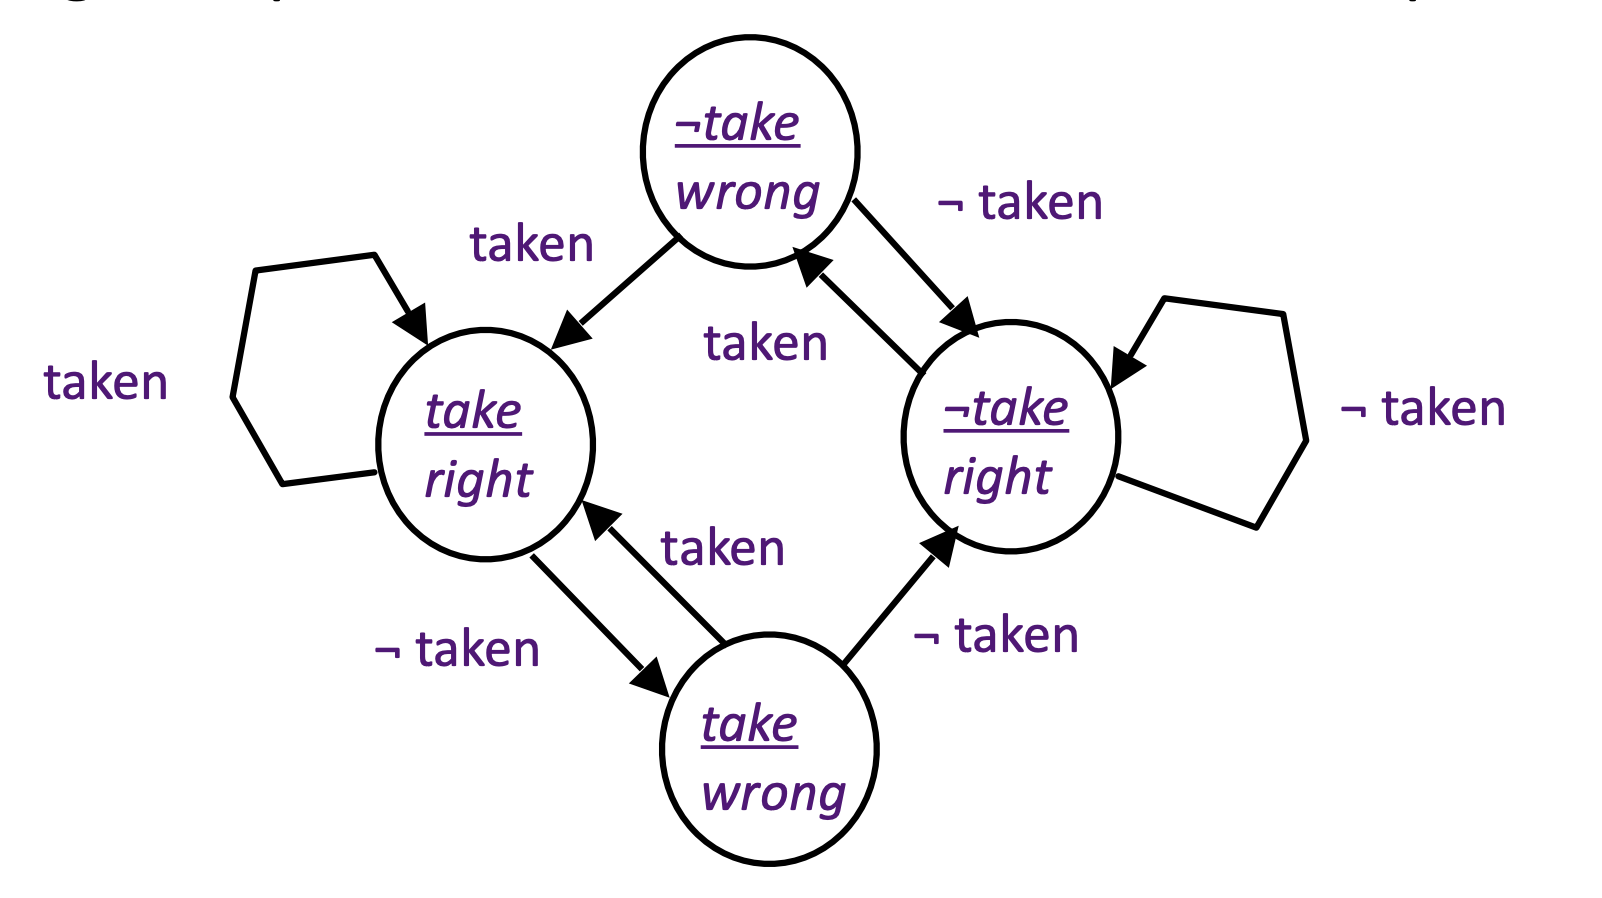
\includegraphics[width=0.5\textwidth]{images/saturating_counter.png}

\caption{State Machine for a Saturating Counter. Source: CS152}
\end{center}
\end{figure}


\newpage
\textbf{BHT / BPB as a Cache}. The branch history table and branch prediction table can be thought of a cache or a buffer. We map each branch instruction by the lower portion of the address into entries of the cache (index into cache by lower address bits). Each cache line contains the saturating counter value that represents history of the instruction. During the guess stage, we check if the cache contains entries of this branch instruction by checking the tag and valid bit. If it is a hit, we read the entry and use the top bit as prediction. 

During the check stage, we read the entry of the cache again to see if behavior of corresponding branch instruction has been recorded. If the entry exists (cache hit) we read and update the current saturating counter based on whether the branch is taken or not, and write back to the cache with updated saturating counter value. If the entry did not exist before, we write a new line in the cache with saturating counter value based on whether the branch was taken or not.


\begin{figure}[hbt]
  \begin{center}
    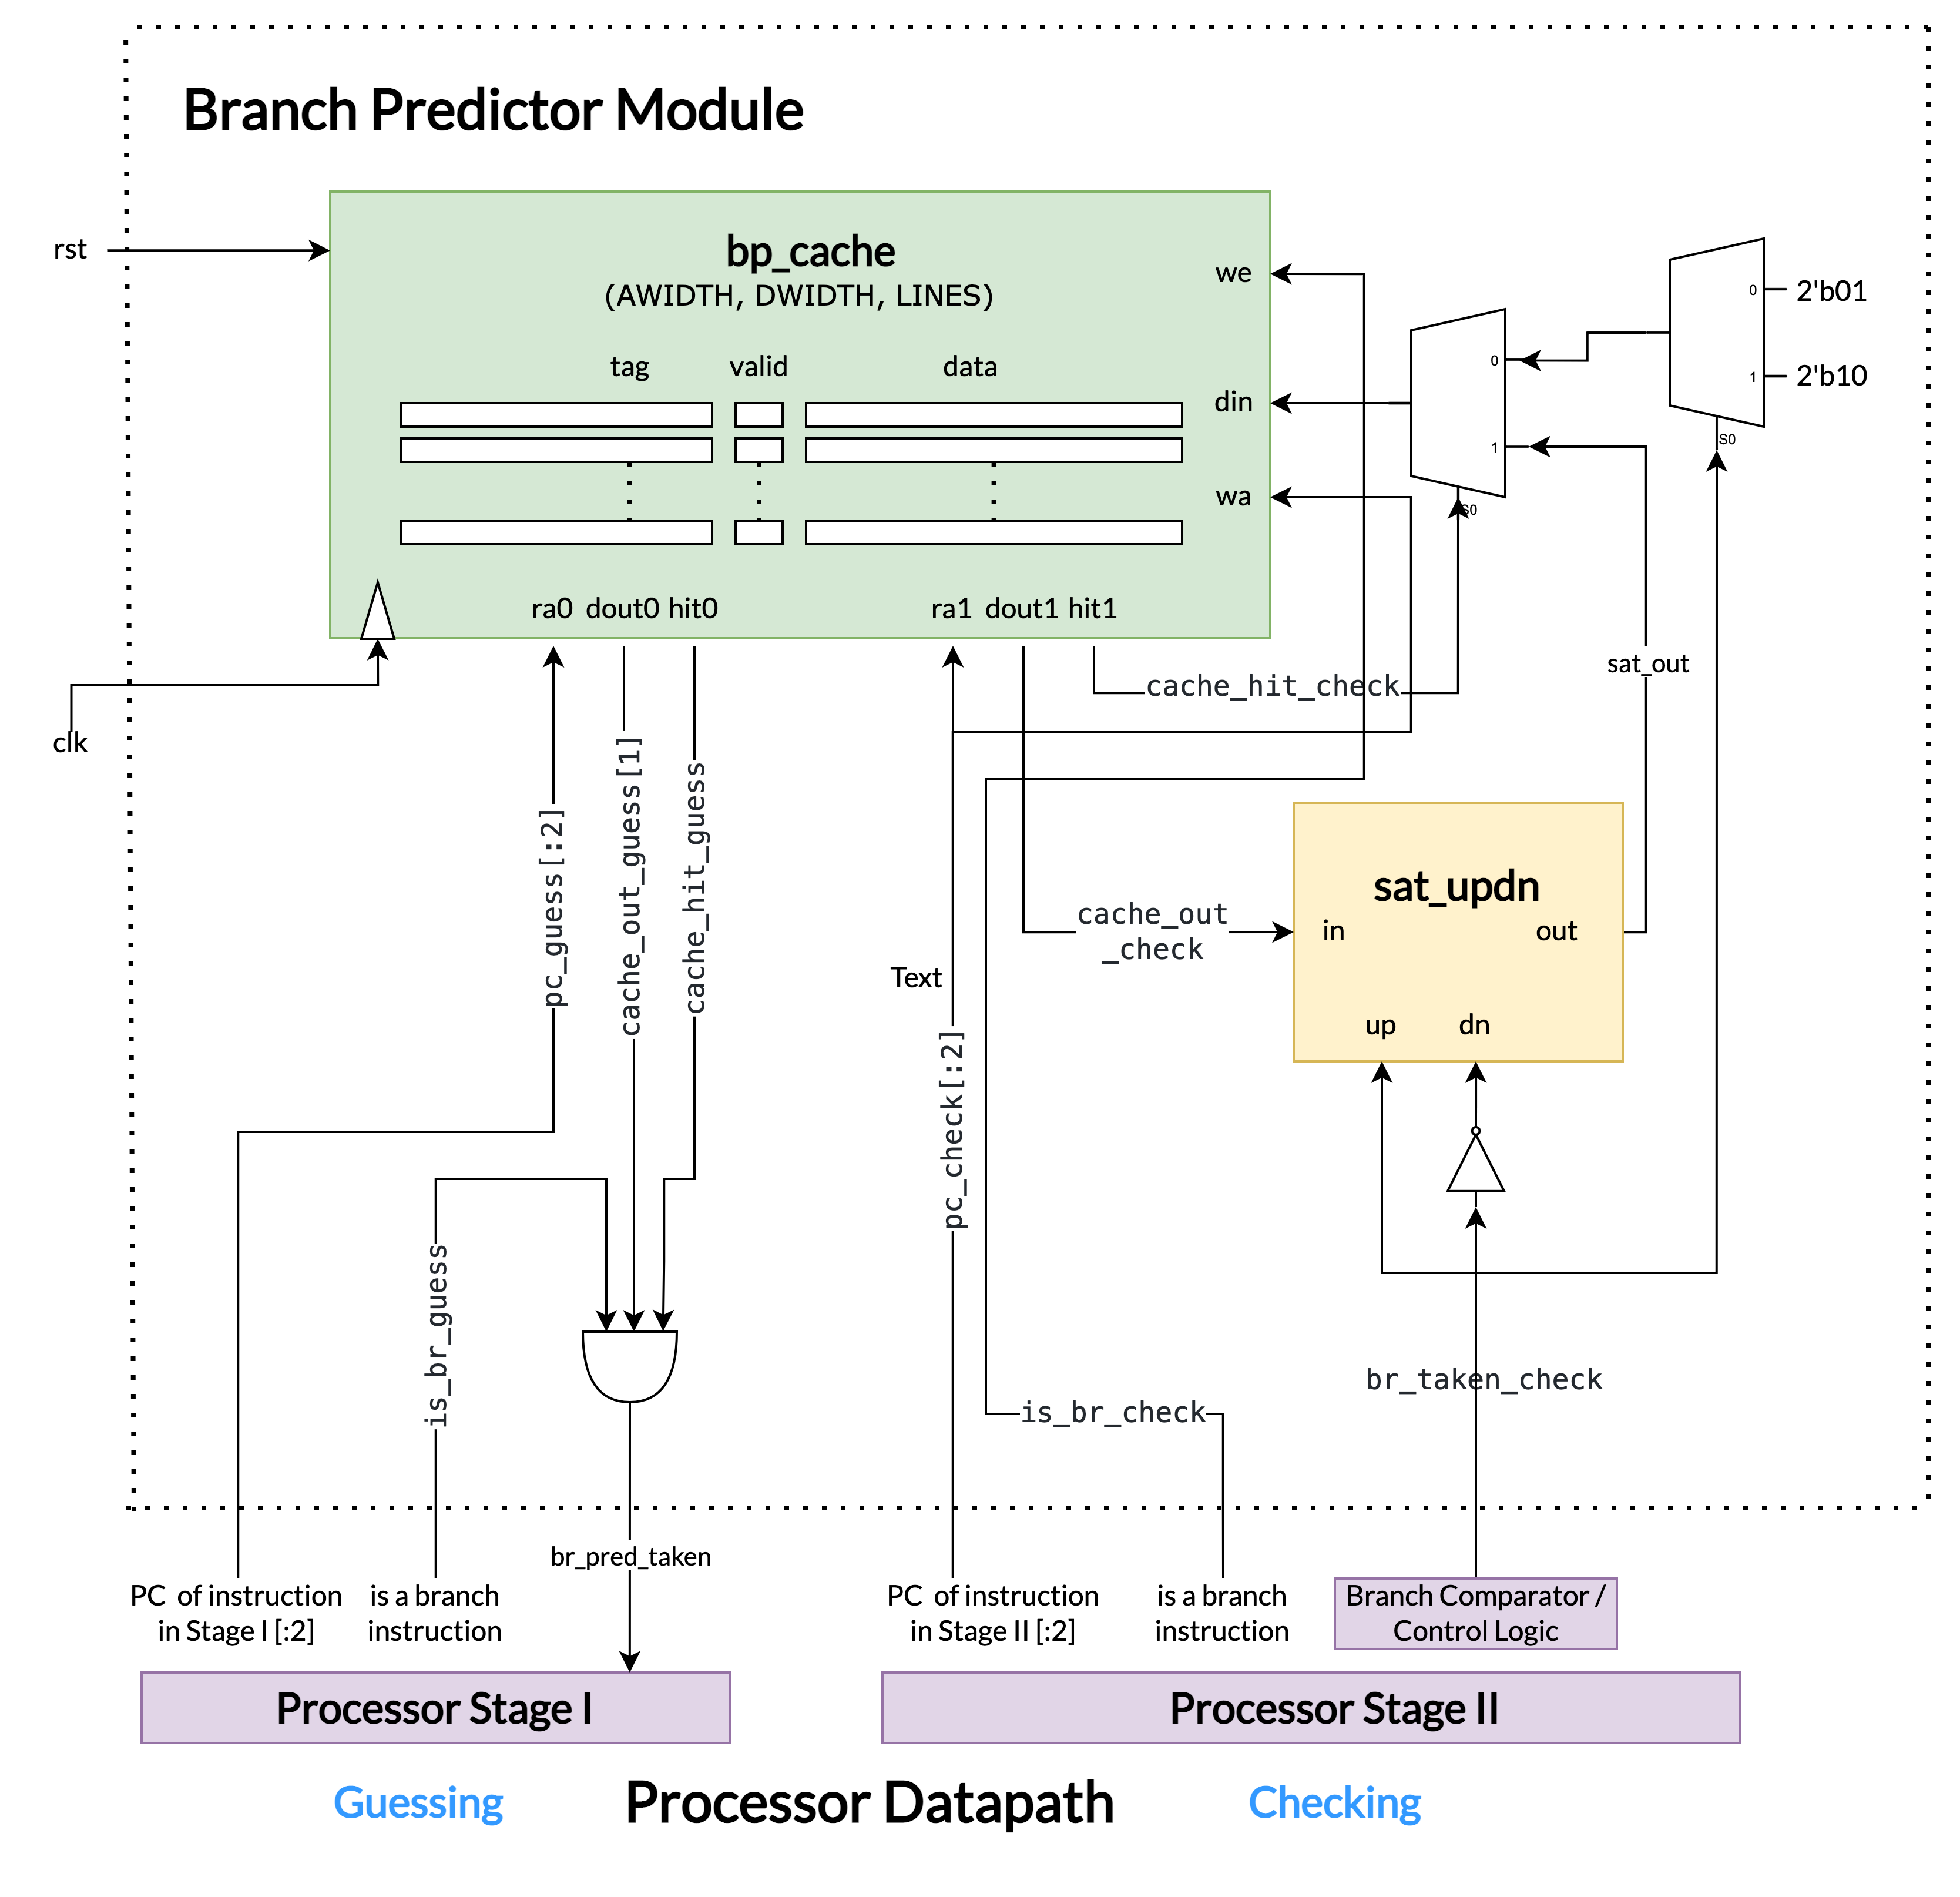
\includegraphics[width=0.9\textwidth]{images/branch_predictor.png}
    \caption{Structure of the Branch Predictor Module; see how the cache, saturating counter composes the branch predictor and how it interacts with signals from Stage I and II of the processor datapath.}
    \label{fig:mem_arch}
  \end{center}
\end{figure}


This formulation treats the BHT just as a regular cache, but with entry that represents a saturating counter which can be used for branch prediction. The diagram below illustrates the module interface our skeleton code provide. We separate the module into a cache and a saturating counter. The cache supports 2 asynchronous reads as we can simultaneously have two branch instructions in flight in Stage I and II. The cache supports 1 synchronous write to update its entry. 

\subsection{Guidelines and requirements}
Please pull the skeleton again before starting this checkpoint. We have added skeleton code in  hardware/src/riscv\_core/branch\_prediction as well as test benches and modifications to other parts of the datapath and software to support adding the branch predictor. Before you start this, make sure you have Checkpoint 2 datapath implemented with naive branch predictor and have mechanism to recover from branch mispredict, as we will solely be replacing naive predictor with a more accurate one.

\begin{enumerate}
  \item Within hardware/src/riscv\_core/branch\_prediction, we have prepared branch\_predictor.v which is the top level branch predictor. It uses components bp\_cache.v and sat\_updn.v which for both you would implement. You do not need to modify branch\_predictor.v. It is important to understand how they all interface with each other, and how you can instantiate and connect the branch\_predictor in your datapath.
  \item Implement a 2-bit \textbf{saturating counter} in sat\_updn.v. Note this should be a purely combination circuit that takes in existing counter value and whether to increment/decrement and compute the new counter value. We do not provide a test bench but we recommend you write one.
  \item Implement the \textbf{cache} in bp\_cache.v, with 2 asynchronous read ports and 1 synchronous write port. Each cache line has tag, valid bit, and fields to store the data. The cache should be parameterizable by address width, data width, and number of cache lines.
  \begin{enumerate}
      \item EECS151 Student should implement a \textbf{direct-mapped} cache.
      \item EECS251A Student should implement either 1) a direct-map and a 2-way set associative cache. 2) a configurable N-way set associative cache. 
    \end{enumerate}
   We will not be providing a test bench for the cache. However, you are \textbf{required} to design a test bench for your cache that covers representative cases such as read miss, read hit, write, eviction, etc (251 students to write test regarding the associativity). You will need to \textbf{explain} your cache testbench to a TA upon checkoff. 
  \item With both saturating counter and cache implemented, you have completed the branch predictor module. We have provided a \textbf{testbench} in hardware/sim/branch\_predictor\_tb.v. This test bench tests your prediction under a series of branches. You branch predictor must \textbf{satisfy} the behavior of this test bench for this checkpoint!
  
  \textit{Note for 251A students:} The final test case in branch\_predictor\_tb tests cache hit/miss after cache line replacement \textbf{assuming a direct-mapped cache}. You will need to update this test case to deal with a 2-way set associative or a configurable N-way set associative cache.
  \item Connect the branch predictor module to the rest of your CPU datapath, with inputs and output in appropriate stages of your CPU (this will vary based on your design). Make sure you still pass all the checkpoint 2 tests so it is still functionally correct. 
  \item To track performance of your branch predictor, we ask you to add two counters, one for \textbf{total} number of branch instructions the CPU encountered, and one for the number of \textbf{correct} predictions. These counters should be mapped as \textbf{Memory Mapped IO} to address 0x8000\_001c and 0x8000\_0020 respectively; they can also be reset similar to cycle and instruction counters. See 2.9.4 Memory Mapped I/O section for updated mapping.  With these stats, you can calculate the \textbf{branch prediction accuracy}. The mmult program has been modified to print those results at the end as well, make sure you recompile it after pulling the changes. 

  We have also provided a testbench in hardware/sim/mmio\_counter\_tb.v, which will run a small set of instructions and print out the MMIO counter values. You may find it helpful to debug branch prediction and MMIO counters here in simulation before testing it on the FPGA. Feel free to add additional test cases.
  \item We connected SWITCH[0] to enable bp\_enable. Once you successfully uploaded the new design to CPU, run mmult with the switch off and on will show the result with branch prediction off / on. The checksum should remain the same but you should see improved performance with branch prediction enabled.
  
\end{enumerate}

\subsection{Checkoff}
\textbf{\branchPredictorTaskName \space materials should be committed to your project repository by \branchPredictorDueDate.}

\begin{itemize}
    \item Pass test bench in hardware/sim/branch\_predictor\_tb.v
    \item Explain your cache test bench design and how that covers all the representative scenarios for your cache to the TA.
    \item Run mmult with branch prediction disabled and enabled by toggling the switch. The program must still be functionally correct with the correct checksum. For both settings, record the CPI, the amount of total branch predictions, the amount of correct branch predictions, and calculate branch prediction accuracy. CPI and branch prediction accuracy must be \textbf{strictly better} with Checkpoint 3 branch predictor pass this checkpoint.
\end{itemize}

\newpage
\section{Checkpoint 4 - Optimization}

Checkpoint 4 is an optimization checkpoint lumped with the final checkoff.
This part of the project is designed to give students freedom to implement the optimizations of their choosing to improve the performance of their processor.
\textbf{251 students must implement branch prediction (details listed in section 4).}

The optimization goal for this project is to minimize the \textbf{execution time} on the \verb|mmult| program, as defined by the 'Iron Law' of Processor Performance.

\begin{equation*}
\frac{\text{Time}}{\text{Program}} = \frac{\text{Instructions}}{\text{Program}} \times \frac{\text{Cycles}}{\text{Instruction}} \times \frac{\text{Time}}{\text{Cycle}}
\end{equation*}

The number of instructions is fixed, but you have freedom to change the CPI and the CPU clock frequency.
Often you will find that you will have to sacrifice CPI to achieve a higher clock frequency, but there also will exist opportunities to improve one or both of the variables without compromises.

\subsection{Grading on Optimization: Frequency vs. CPI}
The bare minimum is that you should improve the achievable frequency of your existing implementation since Checkpoint 2.

You must demonstrate that your processor has a working BIOS, can load and execute \textbf{mmult} (CPI does not need to be less than 1.2).

Full credit will be awarded if you're able to evaluate different design trade-off points (at least three) between frequency and CPI of \textbf{mmult} (especially if you have implemented some interesting optimization for CPI and increase the frequency further would degrade the performance instead of helping).

Also note that your final optimized design does not need to be strictly three-stage pipeline. Extra credit will be awarded based on additional optimizations listed in the extra credit section, please check with a GSI ahead of time if you are expanding to include these. If you have other ideas please check with a GSI to see if it can be awarded extra credit.

A \textbf{very minor} component of the optimization grade is based total FPGA resource utilization, with the best designs using as few resources as possible.
Credit for your area optimizations will be calculated using a cost function.
At a high level, the cost function will look like:
\begin{equation*}
\mathrm{Cost}=\mathrm{C_{LUT}} \times \text{\# of LUTs} + \mathrm{C_{BRAM}} \times \text{\# of Block RAMs} + \mathrm{C_{FF}} \times \text{\# of FFs} + \mathrm{C_{DSP}} \times \text{\# of DSP Blocks}
\end{equation*}
where $\mathrm{C_{LUT}}$, $\mathrm{C_{BRAM}}$, $\mathrm{C_{FF}}$, and $\mathrm{C_{DSP}}$ are constant value weights that will be decided upon based on how much each resource that you use should cost. As part of your final grade we will evaluate the cost of your design based on this metric. Keep in mind that cost is only one very small component of your project grade. Correct functionality is far more important.

\subsection{Clock Generation Info + Changing Clock Frequency}
Open up \verb|z1top.v|.
There's top level input called \verb|CLK_125MHZ_FPGA|.
It's a 125 MHz clock signal, which is used to derive the CPU clock.

Scrolling down, there's an instantiation of \verb|clock_wizard| generated from Vivado, which is a wrapper module of PLL (phase locked loop) primitive on the FPGA.
This is a circuit that can create a new clock from an existing clock with a user-specified multiply-divide ratio.

The \verb|clk_in1| input clock of the PLL is driven by the 125 MHz \verb|CLK_125MHZ_FPGA|.
The frequency of \verb|clk_out1| is calculated as:
\begin{equation*}
  \mathtt{clk\_out1}\_f = \mathtt{clk\_in1}\_f \times \frac{\mathtt{CLKFBOUT\_MULT_F}}{\mathtt{DIVCLK\_DIVIDE} \times \mathtt{CLKOUT0\_DIVIDE}}
\end{equation*}

In our case we get:
\begin{equation*}
  \mathtt{clk\_out1}\_f = 125 \text{ MHz} \times \frac{8}{1 \times 20} = 50 \text{ MHz}
\end{equation*}

You just need to change the local parameter \verb|CPU_CLOCK_PERIOD| in \verb|z1top.v| to set the target clock frequency for your CPU.

\subsection{Critical Path Identification}
After running \verb|make write-bitstream|, timing analysis will be performed to determine the critical path(s) of your design.
The timing tools will automatically figure out the CPU's clock timing constraint based on \verb|CPU_CLOCK_PERIOD| in \verb|z1top.v|.

The critical path can be found by looking in

\verb|z1top_proj/z1top_proj.runs/impl_1/z1top_timing_summary_routed.rpt|.

Look for the paths within your CPU.

For each timing path look for the attribute called ``slack''.
Slack describes how much extra time the combinational delay of the path has before the rising edge of the receiving clock.
It is a setup time attribute.
Positive slack means that this timing path resolves and settles before the rising edge of the clock, and negative slack indicates a setup time violation.

There are some common delay types that you will encounter.
\verb|LUT| delays are combinational delays through a LUT.
\verb|net| delays are from wiring delays. They come with a fanout attribute which you should aim to minimize.
Notice that your logic paths are usually dominated by routing delay; as you optimize, you should reach the point where the routing and LUT delays are about equal portions of the total path delay.

\subsubsection{Schematic View}
To visualize the path, you can open the Vivado project \verb|z1top_proj/z1top_proj.xpr|.
Click \textit{Open Implemented Design} after the implementation to open the Device Floorplan view.
Navigate (on the Timing pane at the bottom) to \verb|Intra-Clock Paths| $\rightarrow$ \verb|cpu_clk| $\rightarrow$ \verb|Setup|.
You can double-click any path to see the logic elements along it, or you can right-click and select \verb|Schematic| to see a schematic view of the path.

The paths in post-PAR timing report may be hard to decipher since Vivado does some optimization to move/merge registers and logic across module boundaries.
You can also use the \href{https://www.xilinx.com/support/answers/54778.html}{\texttt{keep\_hierarchy} attribute} to prevent Vivado from 

\begin{minted}{verilog}
// in z1top.v
(* keep_hierarchy="yes" *) Riscv151 #( ) cpu ( );
\end{minted}

\subsubsection{Finding Actual Critical Paths}
When you first check the timing report with a 50 MHz clock, you might not see your 'actual' critical path.
50 MHz is easy to meet and the tools will only attempt to optimize routing until timing is met, and will then stop.

You should increase the clock frequency slowly and rerun \verb|make write-bitstream| until you fail to meet timing.
At this point, the critical paths you see in the report are the 'actual' ones you need to work on.

Don't try to increase the clock speed up all the way to 100 MHz initially, since that will cause the routing tool to give up even before it tried anything.

\subsection{Optimization Tips}
As you optimize your design, you will want to try running \verb|mmult| on your newly optimized designs as you go along. You don't want to make a lot of changes to your processor, get a better clock speed, and then find out you broke something along the way.

You will find that sacrificing CPI for a better clock speed is a good bet to make in some cases, but will worsen performance in others.
You should keep a record of all the different optimizations you tried and the effect they had on CPI and minimum clock period; this will be useful for the final report when you have to justify your optimization and architecture decisions.

There is no limit to what you can do in this section.
The only restriction is that you have to run the original, unmodified \verb|mmult| program so that the number of instructions remain fixed.
You can add as many pipeline stages as you want, stall as much or as little as desired, add a branch predictor, or perform any other optimizations.
If you decide to do a more advanced optimization (like a 5 stage pipeline), ask the staff to see if you can use it as extra credit in addition to the optimization.

Keep notes of your architecture modifications in the process of optimization.
Consider, but don't obsess, over area usage when optimizing (keep records though).

\subsection{Checkoff}
Refer to \textbf{4.1}. You will run your new implementation on the FPGA again and will be graded based on the best \verb|mmult| performance you were able to achieve, but \textit{more critically} on how many design points you explored.
\pagebreak

\section{Grading and Extra Credit}
\textbf{All groups must complete the final checkoff by \finalCheckoffDueDate.}
If you are unable to make the deadline for any of the checkpoints, it is still in your best interest to complete the design late, as you can still receive most of the credit if you get a working design by the final checkoff.

\subsection{Checkpoints}
\label{checkoff}
We have divided the project up into checkpoints so that you (and the staff) can pace your progress.
%The due dates are indicated at the end of each checkpoint section, as well as in the \textbf{Project Timeline} (Section \ref{project_timeline}) at the end of this document.

\subsection{Style: Organization, Design}
\label{style}
Your code should be modular, well documented, and consistently styled.
Projects with incomprehensible code will upset the graders.

\subsection{Final Project Report}
Upon completing the project, you will be required to submit a report detailing the progress of your EECS151/251A project.
The report should document your final circuit at a high level, and describe the design process that led you to your implementation.
We expect you to document and justify any tradeoffs you have made throughout the semester, as well as any pitfalls and lessons learned.
Additionally, you will document any optimizations made to your system, the system's performance in terms of area (resource use), clock period, and CPI, and other information that sets your project apart from other submissions.

The staff emphasizes the importance of the project report because it is the product you are able to take with you after completing the course.
All of your hard work should reflect in the project report.
Employers may (and have) ask to examine your EECS151/251A project report during interviews.
Put effort into this document and be proud of the results.
You may consider the report to be your medal for surviving EECS151/251A.

\subsubsection{Report Details}
You will turn in your project report PDF file on Gradescope by \textbf{\finalReportDueDate, 11:59PM}.
The report should be around 8 pages total with around 5 pages of text and 3 pages of figures ($\pm$ a few pages on each), though this is not a strict limit.
Ideally you should mix the text and figures together.

Here is a suggested outline and page breakdown for your report.
You do not need to strictly follow this outline, it is here just to give you an idea of what we will be looking for.

\begin{itemize}
  \item \textbf{Project Functional Description and Design Requirements}. Describe the design objectives of your project.  You don't need to go into details about the RISC-V ISA, but you need to describe the high-level design parameters (pipeline structure, memory hierarchy, etc.) for this version of the RISC-V. ($\approx$ 0.5 page)
  \item \textbf{High-level organization}. How is your project broken down into pieces. Block diagram level-description. We are most interested in how you broke the CPU datapath and control
  down into submodules, since the code for the later checkpoints will be pretty consistent across all groups. Please include an updated block diagram ($\approx$ 1 page).
  \item \textbf{Detailed Description of Sub-pieces}. Describe how your circuits work. Concentrate here on novel or non-standard circuits. Also, focus your attention on the parts of the design that were not supplied to you by the teaching staff. ($\approx$ 2 pages).
  \item \textbf{Status and Results}. What is working and what is not? At what frequency (50MHz or greater) does your design run? Do certain checkpoints work at a higher clock speed while others only run at 50 MHz? Please also provide the area utilization. Also include the CPI and minimum clock period of running \verb|mmult| for the various optimizations you made to your processor. This section is particularly important for non-working designs (to help us assign partial credit). ($\approx$ 1-2 pages).
  \item \textbf{Conclusions}. What have you learned from this experience? How would you do it different next time? ($\approx$ 0.5 page).
  \item \textbf{Division of Labor. This section is mandatory. Each team member will turn in a separate document from this part only}. The submission for this document will also be on Gradescope. How did you organize yourselves as a team. Exactly who did what? Did both partners contribute equally? Please note your team number next to your name at the top. ($\approx$ 0.5 page).
\end{itemize}

When we grade your report, we will grade for clarity, organization, and grammar.
Both team members need to submit the Final Report assignment (same report content, but with different writeup for division of labor) to Gradescope. \textbf{We require your final report to be typeset using tools like \LaTeX, or Markdown, or Google Docs/MS Word/Apple Pages etc., but the file that you turn in must be a single PDF file.}

\subsection{Extra Credit}
\label{extra_credit}
Teams that have completed the base set of requirements are eligible to receive extra credit worth up to 10\% of the project grade by adding extra functionality and demonstrating it at the time of the final checkoff.

The following are suggested projects that may or may not be feasible in one week.
\begin{itemize}
  \item Improve Branch Predictor: Beyond our 2-bit saturating based BHT, you can improve the Branch Predictor from Checkpoint 3. You can come up with improved scheme, such as incorporating making the cache set associative (required for 251A students), incorporating global history, adding a Branch Target Buffer, etc. Whatever you choose to do, you must improve your CPI from checkpoint 3 to qualify for extra credit.
  \item 5-Stage Pipeline: Add more pipeline stages and push the clock frequency past 100MHz
  \item RISC-V M Extension: Extend the processor with a hardware multiplier and divider
  \item Everything 100MHz or beyond: Push the frequency of the full \verb|z1top| to 100MHz or better.
\end{itemize}

When the time is right, if you are interested in implementing any of these, see the staff for more details.

\subsection{Project Grading}
\label{deadlinegrading}

\begin{description}
  \item[70\%] {Functionality} at project due date. You will demonstrate the functionality of your processor during the final interview.
  \item[15\%] {Optimization} at final project due date. This score is contingent on implementing all the required functionality. An incomplete project will receive a zero in this category.
  \item[5\%] {Checkpoint} functionality. You are graded on functionality for each completed checkpoint at the checkpoint deadline. The total of these scores makes up 5\% of your project grade. The weight of each checkpoint's score may vary.
  \item[10\%] {Final report} and {style} demonstrated throughout the project.
\end{description}

Not included in the above tabulations are point assignments for extra credit as discussed above. Extra credit is discussed below:

\begin{description}
  \item[Up to 10\%] Additional functionality. Credit based on additional functionality will be qualified on a case by case basis. Students interested in expanding the functionality of their project must meet with a GSI well ahead of time to be qualified for extra credit. Point value will be decided by the course staff on a case by case basis, and will depend on the complexity of your proposal, the creativity of your idea, and relevance to the material taught.
\end{description}

\newpage

\begin{appendices}
\section{Local Development}
You can build the project on your laptop but there are a few dependencies to install.
In addition to Vivado and Icarus Verilog, you need a RISC-V GCC cross compiler and an \verb|elf2hex| utility.

\subsection{Linux}
A system package provides the RISC-V GCC toolchain (Ubuntu): \verb|sudo apt install gcc-riscv64-linux-gnu|.
There are packages for other distros too.

To install \verb|elf2hex|:
\begin{minted}{bash}
git clone git@github.com:sifive/elf2hex.git
cd elf2hex
autoreconf -i
./configure --target=riscv64-linux-gnu
make
vim elf2hex # Edit line 7 to remove 'unknown'
sudo make install
\end{minted}

\subsection{OSX, Windows}
Download SiFive's GNU Embedded Toolchain \href{https://www.sifive.com/boards}{from here}.
See the 'Prebuilt RISC-V GCC Toolchain and Emulator' section.

After downloading and extracting the tarball, add the \verb|bin| folder to your \verb|PATH|.
For Windows, make sure you can execute \verb|riscv64-unknown-elf-gcc -v| in a Cygwin terminal.
Do the same for OSX, using the regular terminal.

For Windows, re-run the Cygwin installer and install the packages\\\verb|git, python3, python2, autoconf, automake, libtool|.
See \href{https://stackoverflow.com/questions/47168311/cygwin-and-failed-to-run-aclocal-no-such-file-or-directory}{this StackOverflow question} if you need help selecting the exact packages to install.

Clone the \verb|elf2hex| repo \verb|git clone git@github.com:sifive/elf2hex|.
Follow the instructions in the \href{https://github.com/sifive/elf2hex}{elf2hex repo README} to build it from git.
You should be able to run \verb|riscv64-unknown-elf-elf2hex| in a terminal.

\pagebreak
\section{BIOS}
\label{sec:biosinfo}
This section was written by Vincent Lee, Ian Juch, and Albert Magyar.

\subsection{Background}
For the first checkpoint we have provided you a BIOS written in C that your processor is
instantiated with. BIOS stands for Basic Input/Output System and forms the bare bones of the
CPU system on initial boot up. The primary function of the BIOS is to locate, and initialize the
system and peripheral devices essential to the PC operation such as memories, hard drives, and
the CPU cores.

Once these systems are online, the BIOS locates a boot loader that initializes the operating
system loading process and passes control to it. For our project, we do not have to worry about
loading the BIOS since the FPGA eliminates that problem for us. Furthermore, we will not deal
too much with boot loaders, peripheral initialization, and device drivers as that is beyond the
scope of this class. The BIOS for our project will simply allow you to get a taste of how the
software and hardware layers come together.

The reason why we instantiate the memory with the BIOS is to avoid the problem of
bootstrapping the memory which is required on most computer systems today. Throughout the
next few checkpoints we will be adding new memory mapped hardware that our BIOS will
interface with. This document is intended to explain the BIOS for checkpoint 1 and how it
interfaces with the hardware. In addition, this document will provide you pointers if you wish to
modify the BIOS at any point in the project.

\subsection{Loading the BIOS}
For the first checkpoint, the BIOS is loaded into the Instruction memory when you first build it.
As shown in the Checkpoint 1 specification, this is made possible by instantiating your
instruction memory to the BIOS file by building the block RAM with the \verb|bios151v3.hex| file. If you
want to instantiate a modified BIOS you will have to change this .hex file in your block RAM
directory and rebuild your design and the memory.

To do this, simply cd to the \verb|software/bios151v3| directory and make the .hex file by running
“make”. This should generate the .hex file using the compiler tailored to our ISA. The
block RAM will be instantiated with the contents of the .hex file.
When you get your design to synthesize and program the board, open up screen using the
same command from Lab 5:

\verb|screen $SERIALTTY 115200|

or

\verb|screen /dev/ttyUSB0 115200|

Once you are in \verb|screen|, if you CPU design is working correctly you should be able to hit Enter
and a carrot prompt \verb|'>'| will show up on the screen. If this doesn’t work, try hitting the reset
button on the FPGA which is the center compass switch and hit enter. If you can’t get the BIOS
carrot to come up, then your design is not working and you will have to fix it.

\subsection{Loading Your Own Programs}
The BIOS that we provide you is written so that you can actually load your own programs for
testing purposes and benchmarking. Once you instantiate your BIOS block RAM with the
\verb|bios151v3.hex| file and synthesize your design, you can transfer your own program files over the
serial line.

To load you own programs into the memory, you need to first have the .hex file for the program
compiled. You can do this by copying the software directory of one of our C programs folders in
/software directory and editing the files. You can write your own MIPS program by writing
test code to the .s file or write your own c code by modifying the .c file.
Once you have the .hex file for your program, impact your board with your design and run:

\verb|hex_to_serial <file name> <target address>|

The \verb|<file name>| field corresponds to the .hex file that you are to uploading to the instruction
memory. The \verb|<target address>| field corresponds to the location in memory you want to write
your program to.

Once you have uploaded the file, you can fire up screen and run the command:

\verb|jal <target hex address>|

Where the \verb|<target hex address>| is where you stored the location of the hex file over
serial. Note that our design does not implement memory protection so try to avoid storing your
program over your BIOS memory. Also note that the instruction memory size for the first
checkpoint is limited in address size so large programs may fail to load.
The jal command will change the PC to where your program is stored in the instruction
memory.

\subsection{The BIOS Program}
The BIOS itself is a fairly simple program and composes of a glorified infinite loop that waits for
user input. If you open the \verb|bios151v3.c| file, you will see that the main method composes of a
large for loop that prints a prompt and gets user input by calling the \verb|read_token| method.
If at any time your program execution or BIOS hangs or behaves unexpected, you can hit the
reset button on your board to reset the program execution to the main method.
The \verb|read_token| method continuously polls the UART for user input from the keyboard until it
sees the character specified by ds. In the case of the BIOS, the termination character
\verb|read_token| is called with is the 0xd character which corresponds to Enter.
The \verb|read_token| method will then return the values that it received from the user. Note that
there is no backspace option so if you make a mistake you will have to wait until the next
command to fix it.

\begin{figure}[H]
  \centering
  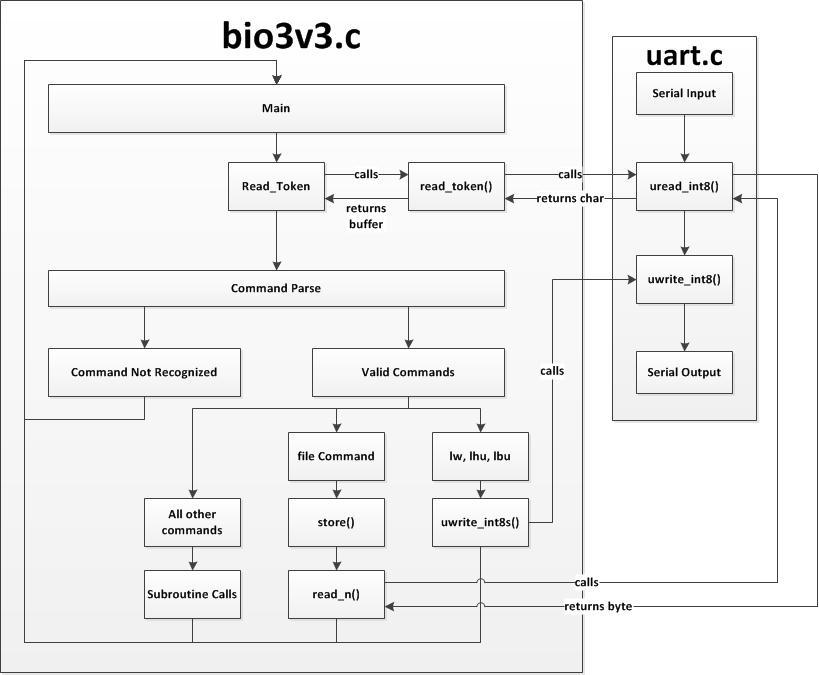
\includegraphics[width=0.7\textwidth]{images/bios_flow.png}
  \caption{BIOS Execution Flow}
\end{figure}

The buffer returned from the \verb|read_token| method with the user input is then parsed by
comparing the returned buffer against commands that the BIOS recognizes. If the BIOS parses a
command successfully it will execute the appropriate subroutine or commands. Otherwise it
will tell you that the command you input is not recognized.
If you want to add commands to the BIOS at any time in the project, you will have to add to the
comparisons that follow after the \verb|read_token| subroutine in the BIOS.

\subsection{The UART}
You will notice that some of the BIOS execution calls will call subroutines in the uart.c file
which takes care of the transmission and reception of byte over the serial line.
The uart.c file contains three subroutines. The first subroutine, \verb|uwrite_int8| executes a
UART transmission for a single byte by writing to the output data register. The second
subroutine \verb|uwrite_int8s| allows you to process an array of type \verb|int8_t| or chars and send
them over the serial line. The third routine \verb|uread_int8| polls the UART for valid data and
reads a byte from the serial line.

In essence, these three routines are operating the UART on your design from a software view
using the memory mapped I/O. Therefore, in order for the software to operate the memory
map correctly, the \verb|uart.c| module must store and load from the correct addresses as defined
by out memory map. You will find the necessary memory map addresses in the uart.h file that
conforms to the design specification.

\subsection{Command List}
The following commands are built into the BIOS that we provide for you. All values are
interpreted in hexadecimal and do not require any radix prefix (ex. ``0x''). Note that there is not
backspace command.

\verb|jal <hexadecimal address>| - Moves program execution to the specified address

\verb|lw <hexadecimal address>| - Displays word at specified address to screen

\verb|lhu <hexadecimal address>| - Displays half at specified address to screen

\verb|lbu <hexadecimal address>| - Displays byte at specified address to screen

\verb|sw <value> <hexadecimal address>| - Stores specified word to address in memory

\verb|sh <value> <hexadecimal address>| - Stores specified half to address in memory

\verb|sb <value> <hexadecimal address>| - Stores specified byte to address in memory

There is another command file in the main() method that is used only when you execute
\verb|hex_to_serial|. When you execute \verb|hex_to_serial|, your workstation will initiate a byte
transfer by calling this command in the BIOS. Therefore, don’t mess with this command too
much as it is one of the more critical components of your BIOS.

\subsection{Adding Your Own Features}
Feel free to modify the BIOS code if you want to add your own features during the project for
fun or to make your life easier. If you do choose to modify the BIOS, make sure to preserve
essential functionality such as the I/O and the ability to store programs. In order to add
features, you can either add to the code in the \verb|bios151v3.c| file or create your own c source and
header files. Note that you do not have access to standard c libraries so you will have to add
them yourself if you need additional library functionality.

\pagebreak
\end{appendices}

\end{document}

